% \iffalse meta-comment
% !TEX program  = pdflatex
% !TEX encoding = utf8
%<*internal>
\iffalse
\fi
\def\nameofplainTeX{plain}
\ifx\fmtname\nameofplainTeX\else
  \expandafter\begingroup
\fi

%</internal>
%<*install>
\input docstrip.tex
\keepsilent
\askforoverwritefalse
\preamble
----------------------------------------------------------------
beilstein -- Support for submissions to the ``Beilstein Journal
of Nanotechnology'' published by the Beilstein-Institut
zur Foerderung der Chemischen Wissenschaften
Version:     2.0
E-mail:      journals-support@beilstein-institut.de
License:     Released under the LaTeX Project Public License v1.3c or later
See          http://www.latex-project.org/lppl.txt
----------------------------------------------------------------

\endpreamble
\postamble

Originally developed by Martin Sievers (info@schoenerpublizieren.de)
Copyright (C) 2009-2020 by Beilstein-Institut zur Foerderung der Chemischen Wissenschaften (Beilstein)

Part of this bundle is derived from cite.sty, to which the
following license applies:
  Copyright (C) 1989-2003 by Donald Arseneau
  These macros may be freely transmitted, reproduced, or
  modified provided that this notice is left intact.

It may be distributed and/or modified under the conditions of
the LaTeX Project Public License (LPPL), either version 1.3c of
this license or (at your option) any later version.  The latest
version of this license is in the file:

   http://www.latex-project.org/lppl.txt

This work has the LPPL maintenancce status "author-maintained".

This work consists of the files beilstein.dtx,
                                CHANGELOG.md,
                                README.md
          and the derived files beilstein.pdf,
                                beilstein.cls,
                                beilstein.ins,
                                bjnano.bst,
                                beilstein-template.tex,
                                beilstein-template.bib.
          Some graphic files for the documentation and template are also added:
                                bjnano_logo.pdf
                                scheme1.pdf
                                scheme2.pdf
                                figure1.pdf
\endpostamble
\usedir{tex/latex/beilstein}
\generate{
  \file{\jobname.cls}{\from{\jobname.dtx}{class}}
}
\usedir{bibtex/bst/beilstein}
\generate{
  \file{bjnano.bst}{\from{\jobname.dtx}{bst}}
}
\nopreamble\nopostamble
\usedir{tex/latex/beilstein}
\generate{
   \file{beilstein-template.tex}{\from{\jobname.dtx}{demo}}
   \file{beilstein-template.bib}{\from{\jobname.dtx}{bib}}
}
%</install>
%<install>\endbatchfile
%<*internal>
\usedir{source/latex/beilstein}
\generate{
  \file{\jobname.ins}{\from{\jobname.dtx}{install}}
}
\ifx\fmtname\nameofplainTeX
  \expandafter\endbatchfile
\else
  \expandafter\endgroup
\fi
%</internal>
%<*driver>
\ProvidesFile{beilstein.dtx}%
[2020/02/22 v2.0 Bundle for submissions to the\MessageBreak ``Beilstein Journal
   of Nanotechnology'' (BJNANO)]
\documentclass[a4paper]{ltxdoc}
\usepackage[american]{babel}
\usepackage{graphicx}
\usepackage[utf8]{inputenc}
\usepackage[T1]{fontenc}
\usepackage{lmodern}
\usepackage{amsmath,amssymb}
\usepackage{array,booktabs,tabularx,longtable}
\usepackage{fancyhdr}
\pagestyle{fancy}
\lfoot{\footnotesize BJNANO Technical Handbook (Version 2.0)}
\cfoot{}
\rfoot{\thepage}
\rhead{\small\rightmark}
\lhead{\small\leftmark}
\usepackage[final]{listings}
\usepackage[onehalfspacing]{setspace}
\usepackage{xspace}
\usepackage[svgnames]{xcolor}
%%%\setlength{\parindent}{0pt}
\DeclareFontFamily{U}{eur}{\skewchar\font'177}
\DeclareFontShape{U}{eur}{m}{n}{%
  <-6> eurm5 <6-8> eurm7 <8-> eurm10}{}
\DeclareFontShape{U}{eur}{b}{n}{%
  <-6> eurb5 <6-8> eurb7 <8-> eurb10}{}
\DeclareSymbolFont{ugrf@m}{U}{eur}{m}{n}
\SetSymbolFont{ugrf@m}{bold}{U}{eur}{b}{n}
\DeclareMathSymbol{\upalpha}{\mathord}{ugrf@m}{"0B}
\providecommand*\env[1]{\texttt{#1}}
\providecommand*\file[1]{\texttt{#1}}
\providecommand*\opt[1]{\texttt{#1}}
\providecommand*\pkg[1]{\textsf{#1}}
\usepackage[%
	pdftitle={A LaTeX class for submissions to the ``Beilstein Journal of
   Nanotechnology'' (BJNANO)},
   pdfauthor={Beilstein-Institut zur Foerderung der Chemischen Wissenschaften},
   urlcolor=blue,%
	linktocpage,%
	a4paper,%
   citecolor=blue,%
   linkcolor=blue,%
	colorlinks=true]{hyperref}
\OnlyDescription     % nur Anleitung (ohne Index und History)
\CodelineIndex       % kein Index wenn auskommentiert
\EnableCrossrefs     % kein Index wenn auskommentiert
\RecordChanges       % keine History wenn auskommentiert
\begin{document}
\DeleteShortVerb{\|}
\DocInput{beilstein.dtx}
\end{document}
%</driver>
% \fi
% \CheckSum{0}
% \CharacterTable
%  {Upper-case    \A\B\C\D\E\F\G\H\I\J\K\L\M\N\O\P\Q\R\S\T\U\V\W\X\Y\Z
%   Lower-case    \a\b\c\d\e\f\g\h\i\j\k\l\m\n\o\p\q\r\s\t\u\v\w\x\y\z
%   Digits        \0\1\2\3\4\5\6\7\8\9
%   Exclamation   \!     Double quote  \"     Hash (number) \#
%   Dollar        \$     Percent       \%     Ampersand     \&
%   Acute accent  \'     Left paren    \(     Right paren   \)
%   Asterisk      \*     Plus          \+     Comma         \,
%   Minus         \-     Point         \.     Solidus       \/
%   Colon         \:     Semicolon     \;     Less than     \<
%   Equals        \=     Greater than  \>     Question mark \?
%   Commercial at \@     Left bracket  \[     Backslash     \\
%   Right bracket \]     Circumflex    \^     Underscore    \_
%   Grave accent  \`     Left brace    \{     Vertical bar  \|
%   Right brace   \}     Tilde         \~}
%
% \changes{v1.0}{2010/05/11}{Release on start of BJNANO public website}
% \changes{v1.1}{2010/08/16}{Page number bug fix}
% \changes{v1.2}{2017/08/16}{Fix for recent babel versions}
% \changes{v1.2}{2017/08/16}{Fix for @misc bib entries}
% \changes{v1.2}{2017/08/16}{All files converted to UTF-8}
% \changes{v1.2}{2017/08/21}{Fix for the declaration of \cs{-} as a robust
% command. There is a conflict between package bpchem and the latest
% \LaTeX{} release}
% \changes{v1.3}{2017/11/09}{Fix: Loading of \pkg{cleveref} is postponed to the
% very end of the preamble in order to avoid problems with \pkg{hyperref}}
% \changes{v1.4}{2018/01/20}{Add new manuscript type \opt{suppinfo}}
% \changes{v1.5}{2019/10/30}{Add new environment \env{funding}}
% \changes{v1.5}{2019/09/12}{Update documentation}
% \changes{v2.0}{2020/02/05}{Update documentation}
% \changes{v2.0}{2020/02/05}{New font scheme: \pkg{newtxtext}, \pkg{newtxtt}
% and \pkg{newtxmath}}
% \changes{v2.0}{2020/02/05}{utf8 is now the standard encoding for
% \pkg{inputenc}}
% \changes{v2.0}{2020/02/05}{CODEN strings were removed from the BiBTeX style
% file}
% \changes{v2.0}{2020/02/11}{Add support for doi in @www}
% \GetFileInfo{\jobname.dtx}
% \DoNotIndex{\newcommand,\newenvironment}
% \DoNotIndex{\def,\edef,\gdef,\xdef,\global,\long,\let}
% \DoNotIndex{\expandafter,\string,\the,\ifx,\else,\fi}
% \DoNotIndex{\csname,\endcsname,\relax,\begingroup,\endgroup}
% \DoNotIndex{\DeclareTextCommand,\DeclareTextCompositeCommand}
% \DoNotIndex{\space,\@empty,\special,\@nil,\advance\@nnil}
% \DoNotIndex{\\,\@gobble,\@@,\@fornoop,\@fortmp,\@ifundefined}
% \DoNotIndex{\@tempcnta,\@tempcntb,\{,\},\alph,\bgroup,\egroup}
% \DoNotIndex{\do,\end,\HN,\ifcase,\ifnum,\IfFileExists,\ifvmode}
% \DoNotIndex{\ignorespaces,\immediate,\input,\item,\jobname}
% \DoNotIndex{\leavevmode,\loop,\repeat,\makeatletter,\makeatother}
% \DoNotIndex{\meaning,\newcounter,\next,\or,\par,\renewcommand}
% \DoNotIndex{\renewcommand,\renewenvironment,\stepcounter}
% \DoNotIndex{\Tg,\thepage,\unskip,\write,\advance,\{,\}}
% \makeatletter
% \newcommand*\DescribeOption{^^A
%  \leavevmode^^A
%  \@bsphack
%  \begingroup^^A
%    \MakePrivateLetters^^A
%    \Describe@Option^^A
% }^^A
% \newcommand*\Describe@Option[1]{^^A
%    \endgroup^^A
%  \marginpar{^^A
%    \raggedleft^^A
%    \PrintDescribeEnv{#1}^^A
%  }^^A
%  \SpecialOptionIndex{#1}^^A
%  \@esphack
%  \ignorespaces
% }%
% \newcommand*\SpecialOptionIndex[1]{^^A
%  \@bsphack
%  \index{^^A
%    #1\actualchar{\protect\ttfamily#1} (option)\encapchar usage^^A
%  }^^A
%  \index{^^A
%    options:\levelchar#1\actualchar{\protect\ttfamily#1}
%    \encapchar usage^^A
%  }^^A
%  \@esphack
% }
%
%^^A For creating examples with nice highlighting of code, and so
%^^A on; based on the system used in the listings source (lstsample).
% \lst@RequireAspects{writefile}
% \newsavebox{\LaTeXdemo@box}
% \lstnewenvironment{LaTeXdemo}[1][code and example]{^^A
%  \global\let\lst@intname\@empty
%  \expandafter\let\expandafter\LaTeXdemo@end
%    \csname LaTeXdemo@#1@end\endcsname
%  \@nameuse{LaTeXdemo@#1}^^A
% }{^^A
%  \LaTeXdemo@end
% }
% \newcommand*\LaTeXdemo@new[3]{^^A
%  \expandafter\newcommand\expandafter*\expandafter
%    {\csname LaTeXdemo@#1\endcsname}{#2}^^A
%  \expandafter\newcommand\expandafter*\expandafter
%    {\csname LaTeXdemo@#1@end\endcsname}{#3}^^A
% }
% \lstdefinestyle{numbers}{numbers=left, stepnumber=1, numberstyle=\tiny, numbersep=5pt}
% \newcommand*\LaTeXdemo@common{^^A
%  \lstset{
%	  style=numbers,
%    basicstyle   = \small\ttfamily,
%    basewidth    = 0.51em,
%    gobble       = 3,
%    frame        = single,
%    framexleftmargin  = -5.4pt,
%    framexrightmargin = -5.4pt,
%    language     = [LaTeX]{TeX},
%    moretexcs    = {
%      affiliation,
%      background,
%      celsius,
%      chem,
%      CN,
%      conclusion,
%      fnnormal,
%		 fnpara,
%      includegraphics,
%      keywords,
%      maketitle,
%      results,
%      sglcolscheme,
%      sifile,
%      text,
%      unit},%
%    texcsstyle   = *\color{blue},
%    frame        = single,
%    backgroundcolor = \color{yellow!60},
%    framesep     = 5pt,
%    upquote
%  }^^A
% }
% \newcommand*\LaTeXdemo@input{^^A
%  \MakePercentComment
%  \catcode`\^^M=10\relax
%  \small
%  \begingroup
%    \setkeys{lst}{
%      SelectCharTable=\lst@ReplaceInput{\^\^I}{\lst@ProcessTabulator}
%    }^^A
%    \leavevmode
%      \input{\jobname.tmp}^^A
%  \endgroup
%  \MakePercentIgnore
% }
% \LaTeXdemo@new{code and example}{^^A
%  \setbox\LaTeXdemo@box=\hbox\bgroup
%    \lst@BeginAlsoWriteFile{\jobname.tmp}^^A
%    \LaTeXdemo@common
% }{^^A
%    \lst@EndWriteFile
%  \egroup
%  \begin{center}
%    \ifdim\wd\LaTeXdemo@box>0.48\linewidth\relax
%      \hbox to\linewidth{\box\LaTeXdemo@box\hss}^^A
%        \begin{minipage}{\linewidth}
%          \LaTeXdemo@input
%        \end{minipage}
%    \else
%      \begin{minipage}{0.48\linewidth}
%        \LaTeXdemo@input
%      \end{minipage}
%      \hfill
%      \begin{minipage}{0.48\linewidth}
%        \hbox to\linewidth{\box\LaTeXdemo@box\hss}^^A
%      \end{minipage}
%    \fi
%  \end{center}
% }
% \LaTeXdemo@new{code only}{^^A
%  \LaTeXdemo@common
% }{^^A
% }%
%
% \newinsert\bx@S
% \newinsert\bx@T
% \newinsert\bx@U
% \newinsert\bx@V
% \newinsert\bx@W
% \newinsert\bx@X
% \newinsert\bx@Y
% \newinsert\bx@Z
% \newinsert\bx@AA
% \newinsert\bx@BB
% \newinsert\bx@CC
% \newinsert\bx@DD
% \newinsert\bx@EE
% \newinsert\bx@FF
% \newinsert\bx@GG
% \newinsert\bx@HH
% \newinsert\bx@II
% \newinsert\bx@JJ
% \gdef\@freelist{\@elt\bx@A\@elt\bx@B\@elt\bx@C\@elt\bx@D\@elt\bx@E
%   \@elt\bx@F\@elt\bx@G\@elt\bx@H\@elt\bx@I\@elt\bx@J
%   \@elt\bx@K\@elt\bx@L\@elt\bx@M\@elt\bx@N
%   \@elt\bx@O\@elt\bx@P\@elt\bx@Q\@elt\bx@R
%   \@elt\bx@S\@elt\bx@T\@elt\bx@U\@elt\bx@V
%   \@elt\bx@W\@elt\bx@X\@elt\bx@Y\@elt\bx@Z
%   \@elt\bx@AA\@elt\bx@BB\@elt\bx@CC\@elt\bx@DD
%   \@elt\bx@EE\@elt\bx@FF\@elt\bx@GG\@elt\bx@HH
%   \@elt\bx@II\@elt\bx@JJ}
%
% \renewcommand*{\fps@table}{htb}
% \setlength\belowcaptionskip{10pt}
%
% \providecommand*\env[1]{\texttt{#1}}
% \providecommand*\file[1]{\texttt{#1}}
% \providecommand*\opt[1]{\texttt{#1}}
% \providecommand*\pkg[1]{\textsf{#1}}
% \newcommand*{\BJNANO}{\emph{Beilstein Journal of Nano\-tech\-nology}\xspace}
% \def\testbx{bx}
% \DeclareRobustCommand*{\chem}[1]{\ensuremath{%
% \ifx\testbx\f@series\mathbf{#1}\else\mathrm{#1}\fi}}
% \DeclareRobustCommand*{\unit}[1]{%
%  \ensuremath{\def\mu{\mbox{\textmu}}\def~{\,}%
%  \unskip~%
%  \ifx\testbx\f@series\mathbf{#1}\else\mathrm{#1}\fi}}
% \renewcommand*\thempfootnote{\@alph\c@mpfootnote}
% \renewcommand\@makefntext[1]%
%     {\noindent\makebox[.5em][l]{\@makefnmark\,}#1}
% \renewcommand{\footnoterule}{}
% \def\BibTeX{\rmfamily B\kern-.05em%
%    \ifx\testbx\f@series{\normalsize I\kern-.025em B\kern-.08em}%
%    \else{\textsc{i\kern-.025em b}\kern-.08em}%
%    \fi%
%    \unskip T\kern-.1667em\lower.7ex\hbox{E}\kern-.125emX}
% \setlength{\columnsep}{1cm}
% \makeatother
%
% \begin{titlepage}
% \setstretch{1.8}
% \renewcommand\thefootnote{\fnsymbol{footnote}}
% \vspace*{-2.5cm}%
% {\includegraphics*[width=7.7cm,keepaspectratio]{bjnano_logo}}\\[1cm]
% \begin{center}
% {\bfseries\LARGE Technical Handbook}\\[3ex]
% {\Large The \LaTeX\ \pkg{Beilstein} bundle for submissions to the\\%
% \emph{Beilstein Journal of Nanotechnology}}
% \end{center}
% \vspace{2cm}
% \setstretch{1.3}
% \begin{multicols}{2}
% \tableofcontents
% \end{multicols}
% \vspace{1cm}
% \begin{abstract}
% \noindent The \pkg{Beilstein} bundle provides a \LaTeX\ class file and a
% \BibTeX\ style file in accordance with the requirements of
% submissions to the \BJNANO. Although the files can be used for any kind of
% document, they have only been designed and tested to be suitable for
% submissions to the \BJNANO.
% \end{abstract}
% \end{titlepage}
% \clearpage
% \section{Introduction}
% The \pkg{Beilstein} bundle consists of three parts. The \LaTeX\ class
% \file{beilstein.cls} is intended to be used for submissions. It is
% based on the standard \pkg{article} class, but was modified
% to meet the requirements for submissions to the \BJNANO as
% published in the ``Instructions for Authors'' \cite{Beilstein-MSG}.
% Moreover the \LaTeX\ class \file{beilstein.cls} facilitates ease of use by
% providing the authors with a set of useful macros and environments.
%
% The \BibTeX\ style \file{bjnano.bst} is used by the class to format
% citations and references correctly. It is based on Joseph Wright's
% \file{achemso.bst}, but was largely adjusted to work exactly on
% \BJNANO submissions.
%
% Finally, an example document is included in the \pkg{Beilstein} bundle. It is
% intended to be used as a template for submissions, and illustrates the
% usage of the class and the \BibTeX\ file.
%
% \section{Installation}
% \subsection{Global installation via your \TeX{} distribution}
% From version 1.2 onwards, the \pkg{Beilstein} bundle is distributed via CTAN
% and the major \TeX{} distributions. Therefore after having updated your \TeX{}
% Live or MiKTeX installation you can use the \pkg{Beilstein} files right away.
%
% \subsection{Local TDS installation}
% The \pkg{Beilstein} bundle is supplied with the TDS-ready ZIP file,
% \file{beilstein-tds.zip}. Simply unzip this file into your local texmf
% tree and run your hash program (e.g., \texttt{texhash} for recent
% \TeX{}Live or MiK\TeX\ systems).
%
% To extract the bundle of files and to build the documentation
% yourself, run pdf\LaTeX\ on \texttt{beilstein.dtx}.
% The files can then be installed either by putting them into the
% current working directory (where the main \TeX\ file is) or --- much
% better --- as described above by moving the files to suitable places
% in a local texmf tree \$LOCALTEXMF according to
% Table~\ref{tab:install}.
% \begin{table}
% \centering
% \caption{Files contained in the \pkg{Beilstein} bundle.}
% \label{tab:install}
% \begin{tabular}{l@{\quad$\rightarrow$\quad}l}
% \toprule
% File & Directory\\\midrule
% \file{beilstein.cls} & \$LOCALTEXMF/tex/latex/beilstein\\
% \file{beilstein.dtx} & \$LOCALTEXMF/source/latex/beilstein\\
% \file{beilstein.ins} & \$LOCALTEXMF/source/latex/beilstein\\
% \file{beilstein-template.bib} & \$LOCALTEXMF/tex/latex/beilstein\\
% \file{beilstein-template.tex} & \$LOCALTEXMF/tex/latex/beilstein\\
% \file{bjnano.bst} & \$LOCALTEXMF/bibtex/bst/beilstein\\
% \file{bjnano\_logo.pdf} & \$LOCALTEXMF/source/latex/beilstein\\
% \file{figure1.pdf} & \$LOCALTEXMF/doc/latex/beilstein\\
% \file{scheme1.pdf} & \$LOCALTEXMF/tex/latex/beilstein\\
% \file{scheme2.pdf} & \$LOCALTEXMF/tex/latex/beilstein\\
% \bottomrule
% \end{tabular}
% \end{table}
%
% \newpage
% If you are not sure about local texmf trees at all, you can have a
% look at \url{https://texfaq.org/FAQ-inst-wlcf} for more information.
%
% \section{Requirements}
% The \pkg{Beilstein} class was designed to rely on standard \LaTeX\
% packages only. It requires the following ones:
% \begin{itemize}
% \item Internal packages
% \begin{itemize}
%  \item \pkg{xkeyval},
%  \item \pkg{ifthen},
%  \item \pkg{babel},
%  \item \pkg{inputenc, fontenc}.
% \end{itemize}
% \item Fonts
% \begin{itemize}
%  \item \pkg{newtxtext}, \pkg{tgheros}, \pkg{newtxtt}
%  \item \pkg{textcomp}.
% \end{itemize}
% \item Page layout
% \begin{itemize}
%  \item \pkg{geometry},
%  \item \pkg{ragged2e}, \pkg{everysel}, \pkg{footmisc},
%  \item \pkg{setspace},
%  \item \pkg{lineno}.
% \end{itemize}\pagebreak
% \item Math and science
% \begin{itemize}
%  \item \pkg{amsmath, amstext, amssymb, amsgen, amsbsy, amsopn, amsfonts,
% newtxmath}.
% \end{itemize}
% \item Floats
% \begin{itemize}
%  \item \pkg{float},
%  \item \pkg{flafter},
%  \item \pkg{graphicx},
%  \item \pkg{array},
%  \item \pkg{tabularx},
%  \item \pkg{longtable}.
% \end{itemize}
% \item Bibliography
% \begin{itemize}
%  \item \pkg{natbib}.
% \end{itemize}
% \end{itemize}
%
% All these packages should be present in any major \TeX\
% distribution and are also available from \emph{The Comprehensive
% TeX Archive Network} (CTAN) at \url{https://www.ctan.org}.
%
% A complete list of used files and tested versions can be found in
% the Appendix section on page~\pageref{appendix}.
%
% \section{The class file}
% \subsection{Class options}
% Most of the things to be considered for submissions to the \BJNANO are
% directly included into the class file. There is only one major choice authors
% have to make, i.e., to determine the type of manuscript they
% want to submit.
%
% \DescribeOption{manuscript=}%
% The Beilstein-Institut has defined five such types and each type
% has a special purpose and structure. The chosen option is used
% internally to check for mandatory sections and elements. The types are
% designed to give the author a slight control over the article structure.
%
% The selection of the type is done by the key-value-option \opt{manuscript},
% which can take the values listed in Table~\ref{tab:optionsmanuscript}.
% To switch your document to a ``Book Review Article'' e.g.,
% simply use \cs{documentclass[manuscript=bookreview]\{beilstein\}}.
% In case of an unknown value, the class will use the default option.
%
% \begin{table}
% \centering
% \caption{Possible values for key-value option
% ``manuscript''.\textsuperscript{\textit{a}}}
% \label{tab:optionsmanuscript}
% \begin{tabular}{ll}
% \toprule
% Option & Meaning\\\midrule
% \opt{manuscript=bookreport} & Book Report Article\\
% \opt{manuscript=commentary} & Commentary Article\\
% \itshape\opt{manuscript=fullresearchpaper} &
% \itshape Full Research Paper\\
% \opt{manuscript=letter} &
% Letter Article\\
% \opt{manuscript=review} & Review Article\\
% \opt{manuscript=suppinfo} & Supporting Information\\
% \bottomrule
% \end{tabular}\\
% \begin{flushleft}\footnotesize
% \textsuperscript{\textit{a}}Default option is printed in italics.
% \end{flushleft}
% \end{table}
% \newpage
%
% \DescribeOption{american}\DescribeOption{british}
% Two other options of a more technical aspect exist. Firstly, you can
% tell \LaTeX\ whether you use American or British English (see
% Table~\ref{tab:language}).
% Internally only different hyphenation patterns are used. So you might not see
% a difference in the output at first sight.
% \begin{table}
% \centering
% \caption{Options for language.\textsuperscript{\textit{a}}}
% \label{tab:language}
% \begin{tabular}{ll}
% \toprule
% Option & Meaning\\\midrule
% \itshape \opt{american}, \opt{USenglish} & \itshape Use American English\\
% \opt{british}, \opt{english}, \opt{UKenglish} & Use British English\\
% \bottomrule
% \end{tabular}\\
% \begin{flushleft}\footnotesize
% \textsuperscript{\textit{a}}Default option is printed in italics.
% \end{flushleft}
% \end{table}
%
% \DescribeOption{applemac}\DescribeOption{latin1}%
% \DescribeOption{utf8}%
% Secondly, you might want to change the input encoding of your
% document, e.g., when using accented characters. Therefore, the class
% offers a small set of options (see Table~\ref{tab:inputenc}). The option
% \opt{utf8} is set as default beginning with version 2.0.
% \begin{table}
% \centering
% \caption{Options for input encoding.%\textsuperscript{\textit{a}}}
% \label{tab:inputenc}
% \begin{tabular}{ll}
% \toprule
% Option & Meaning\\\midrule
% \opt{applemac} & Use special Mac encoding\\
% \opt{latin1} & Use ISO8859-1 encoding\\
% \itshape \opt{utf8} & \itshape Use UTF-8 encoding\\
% \bottomrule
% \end{tabular}\\
% \begin{flushleft}\footnotesize
% \textsuperscript{\textit{a}}Default option is printed in italics.
% \end{flushleft}
% \end{table}
%
% \noindent Further options have been added to the recent version of the class:%
%
% \DescribeOption{sectionnumbering}%
% The \pkg{Beilstein} class disables the usual section numbering
% mechanism by changing the counter ``secnumdepth'' appropriately. You
% can switch back by using the class option \opt{sectionnumbering=true} or
% just \opt{sectionnumbering}. Doing so all non-starred sectioning commands
% will be numbered while the starred versions still have no number.
%
% \DescribeOption{fnpara}
% By default footnotes can only be used in tables and are printed one
% per line. This can be changed to paragraph mode, either locally (see
% page~\pageref{pg:fnpara}) or globally. To this purpose the \pkg{Beilstein}
% class offers the option \opt{fnpara=true} or just \opt{fnpara}.
%
% \DescribeOption{Global options}
% The \pkg{Beilstein} class was developed to include all necessary
% requirements. However, if you need extra options for
% packages already being loaded by the class itself, you can add them
% to the list of global options.
%
% \subsection{Title page}
% The \BJNANO has its own title page format. However,
% a more or less standard set of \LaTeX\ commands can be used to provide the
% necessary information right after \cs{begin\{document\}}:
%
% \DescribeMacro{\title}
% The title of your manuscript is given with \cs{title\marg{title}}.
% There is also an optional argument that can be used when writing
% a document for the Supporting Information, e.g.,
% \cs{title\oarg{sititle}\marg{title}}. Both information are
% automatically used on the title page of the Supporting Information.
% For more information about creating Supporting Information files
% please see page~\pageref{suppinfo}.
%
% \DescribeMacro{\sititle}
% As an alternative to the optional argument of \cs{title}
% you can use the macro \cs{sititle\marg{sititle}}.
%
% \DescribeMacro{\author}\DescribeMacro{\author*}
% Each author of the article is named within their own \cs{author}
% command. For a corresponding author the extended version
% \cs{author*} must be used. It has an additional second mandatory
% argument holding the author's email address.
%
% With both commands the author's name is printed followed by a superscript
% number for the appropriate affiliation(s). As these numbers can be the same
% for several authors, an optional argument for a specific number can
% be used:\\
% \cs{author\oarg{affiliation number}\marg{author's name}} or\\
% \cs{author*\oarg{affiliation number}\marg{author's name}\marg{email
% address}}.
%
% If you want to provide an email address for a non-corresponding author,
% there is a second optional argument:\\
% \cs{author\oarg{affiliation number}\oarg{email address}\marg{author's name}}
%
% \vspace{0.3em}
% \noindent\fcolorbox{black}{red!40}{\parbox{%
% \dimexpr\textwidth-2\fboxsep-2\fboxrule\relax}{
% In order to add an email address the first optional argument
% has to be present in any case. If there is no affiliation number, empty
% square brackets need to be given.}}
%
% \vspace{0.3em}
% \DescribeMacro{\affiliation}
% The affiliations are given with \cs{affiliation\marg{postal address}}
% and are numbered consecutively. Each \cs{author} with dedicated affiliation(s)
% is followed by one or more \cs{affiliation} commands (see example
% below). This can also be combined with the optional affiliation number.
%
% \DescribeMacro{\maketitle}
% To print the title page use the command
% \cs{maketitle}.
% A complete title block might look like this:
% \begin{LaTeXdemo}[code only]
%   \begin{document}
%   \title{Synthesis of highly substituted allenylsilanes by
%      alkylidenation of silylketenes}
%   %Corresponding author:
%   \author*{Stephen P. Marsden}{s.p.marsden@leeds.ac.uk} %
%   \affiliation{School of Chemistry, University of Leeds, Leeds
%      LS2 9JT, United Kingdom}
%   %A second author with two affiliations and an email address:
%   %Important: empty first optional argument
%   \author[][Ducept@...]{Pascal C. Ducept}
%   \affiliation{Department of Chemistry, Imperial College London,
%      London SW7 2AY, United Kingdom}
%   \affiliation{An alternative address can be given here.}
%   %A third author with the same affiliation as the second:
%   \author[2]{X. Y.}
%   \maketitle %print the title page
% \end{LaTeXdemo}
%
% For abstract and keywords please see section~\ref{sec:special}.
%
% \subsection{Section headers}
% You can use the standard \LaTeX\ sectioning commands (with the exception of
% \cs{chapter}) to structure your document. Depending on the type of
% manuscript some sections are mandatory while others are optional.
%
% For a ``Full Research Paper'' the following section headings might
% be used:
% \begin{LaTeXdemo}[code only]
%   \section{Introduction}
%   ...
%   \section{Experimental}
%   ...
%   \section{Results and Discussion}
%   ...
%   \section{Conclusion}
% \end{LaTeXdemo}
%
% Table \ref{tab:specialsections} gives an overview of all allowed section
% headings for the different \pkg{Beilstein} class manuscript types.
% \clearpage
% \begin{table}
% \centering
% \begin{minipage}{\linewidth}
% \caption{Allowed section headings for the different \pkg{Beilstein} class
% manuscript types.}
% \label{tab:specialsections}
% \begin{tabular}{@{}l*{5}{>{$}c<{$}}@{}}
% \toprule
% Section heading& \multicolumn{5}{c@{}}{Manuscript
%  type\textsuperscript{\textit{a}}}\\
% &\mbox{BR}\textsuperscript{\textit{b}} & \mbox{CA}%
%  \textsuperscript{\textit{c}}&\mbox{FR}\textsuperscript{\textit{d}}&
% \mbox{LA}\textsuperscript{\textit{e}} & \mbox{RA}%
%  \textsuperscript{\textit{f}}\\\midrule
% \texttt{Book Details} & + & - & - & - & - \\
% \texttt{Conclusion}   & - & + & o & - & + \\
% \texttt{Discussion}   & - & + & - & - & - \\
% \texttt{Experimental} & - & - & o & - & - \\
% \texttt{Findings}     & - & - & - & + & - \\
% \texttt{Introduction} & - & + & + & - & - \\
% \texttt{Main Text}    & + & - & - & - & - \\
% \texttt{Results and Discussion} (may be separate) & - & - & + & - & - \\
% \texttt{Review}       & - & - & - & - & + \\
% \bottomrule
% \end{tabular}
% \begin{flushleft}\footnotesize
% \textsuperscript{\textit{a}}$+$ denotes a mandatory, $o$ an optional and $-$ a
%  non-feasible section\\
% \textsuperscript{\textit{b}}Book Report Article\\
% \textsuperscript{\textit{c}}Commentary Article\\
% \textsuperscript{\textit{d}}Full Research Paper\\
% \textsuperscript{\textit{e}}Letter Article\\
% \textsuperscript{\textit{f}}Review Article\\
% \end{flushleft}
% \end{minipage}
% \end{table}
%
% \subsection{Special sections}\label{sec:special}
% \DescribeEnv{abstract}
% After the title page an abstract must be given (with the exception of
% ``Book Reports'' and ``Commentaries''). To meet the specifications for
% \BJNANO submissions \LaTeX\ redefines the usual \env{abstract} environment
% internally.
%
% \DescribeMacro{\keywords}
% The ``Keywords'' need to be given right after the abstract. There can be an
% arbitrary number of keywords (at least five keywords are recommended), and
% therefore the \cs{keywords} macro has only one mandatory argument holding the
% keywords separated by semicolons.
%
% An abstract with keywords should look like this:
% \begin{LaTeXdemo}[code only]
%   \begin{abstract}
%  		...
%   \end{abstract}
%   \keywords{allenylsilanes; rhodium(II) octanoate-mediated
%      rearrangement; silylketenes; titanium carbenoids; ylide}
% \end{LaTeXdemo}
% \clearpage
%
% \DescribeEnv{acknowledgements}
% \DescribeEnv{funding}
% The sections ``Acknowledgements'' and ``Funding'' are optional parts of all
% article types.
%
% \vspace{0.3em}
% \noindent\fcolorbox{black}{red!40}{\parbox{%
% \dimexpr\textwidth-2\fboxsep-2\fboxrule\relax}{%
% All financial disclosures are supposed to be part of the ``Funding''
% section.}}
%
% As the layout differs from that of the main text, these sections should be
% written using the environments \env{acknowledgements} and \env{funding}:
%
% \begin{LaTeXdemo}[code only]
%   \begin{acknowledgements}
%   We would like to thank ...
%   \end{acknowledgements}
% \end{LaTeXdemo}
%
% \begin{LaTeXdemo}[code only]
%   \begin{funding}
%   This work was financially supported by ...
%   The authors are grateful for funding from ...
%   \end{funding}
% \end{LaTeXdemo}
%
% \DescribeEnv{suppinfo}\label{suppinfo}%
% Another optional section of an article is the
% ``Supporting Information'', which may consist of various ``Supporting
% Information Files''. To begin this section simply use \cs{begin\{suppinfo\}}.
%
% \DescribeMacro{\sifile}
% Inside the \env{suppinfo} environment the command \cs{sifile} is
% used to add a ``Supporting Information File''. The syntax is:\\
% \cs{sifile\oarg{long description}\marg{filename}\marg{format}\marg{short
% description}}
%
% Each \cs{sifile} can be followed by a \cs{label\marg{labelname}} to
% cross-reference that file in the main text using
% \cs{ref\marg{labelname}}.
%
% The complete section could look like this:
% \begin{LaTeXdemo}[code only]
%   \begin{suppinfo}
%   \sifile{experimental_part.pdf}{PDF}{Experimental part}
%   \label{si:experimental-part}
%   \sifile[A long description about the experimental data given in
%      this file]{nmr1.pdf}{PDF}{NMR spectra of compounds \CN{1},
%      \CN{2}, \CN{6} and \CN{7}.}
%   \end{suppinfo}
% \end{LaTeXdemo}
%
% \DescribeEnv{\LaTeX\ source}A Supporting Information File can be created from
% a \LaTeX\ source using the Beilstein  \LaTeX\ class. The same syntax that is
% used for the title page of the main manuscript can be used for the
% Supporting Information. An additional title for the
% Supporting Information (e.g., ``Additional experimental data'') can be added
% by using the \oarg{sititle} option of the \cs{title} command:
% \cs{title\oarg{sititle}\marg{manuscript title}}.\\
% \DescribeMacro{\sititle}
% Alternatively, the macro \cs{sititle\marg{sititle}} can be used.
%
% \subsection{Floats}\label{sec:floats}
% \DescribeEnv{figure}
% \DescribeEnv{table}
% \DescribeEnv{scheme}
% In addition to the environments \env{table} and \env{figure} already included
% in \LaTeX , there is a third environment for \BJNANO publications, i.e.,
% \env{scheme}. There is no difference in usage between \env{scheme}
% and the former two. To add a scheme ``AScheme.pdf'' you can enter the
% following:
% \begin{LaTeXdemo}[code only]
%   \begin{scheme}
%   \caption{A scheme demonstrating something.}
%   \label{scheme:something}
%   \includegraphics[width=16.8cm,keepaspectratio]{AScheme}
%   \end{scheme}
% \end{LaTeXdemo}
%
% \noindent\fcolorbox{black}{red!40}{\parbox{%
% \dimexpr\textwidth-2\fboxsep-2\fboxrule\relax}{%
% pdf\LaTeX\ is limited to a small set of graphic formats. All files have
% to be either in the PDF, PNG or JPG format.\\
% Using EPS graphics will lead to an error during upload to the submission
% system. EPS graphics need to be converted to PDF, e.g., by using the package
% \pkg{epstopdf}, before uploading the manuscript to the submission system.}}
%
% \vspace{\baselineskip}
% \DescribeMacro{\caption}\DescribeMacro{\label}
% Please note that it does not matter whether \cs{caption} is put above or
% below \cs{includegraphics}. The caption will always be below the scheme in
% the output file. The same mechanism is used to put figure captions
% below and table captions above the content. If you want to add a
% concise title to a float, please use the optional argument:
% \cs{caption\oarg{concise title}\marg{legend}}.
% \DescribeMacro{\ref}
% However, as common in \LaTeX\ \cs{label\marg{labelname}} must
% always follow \cs{caption}, otherwise a corresponding \cs{ref}
% command will yield wrong results.
%
% \DescribeMacro{\sglcolfigure}
% \DescribeMacro{\sglcolscheme}
% \DescribeEnv{sglcoltabular}\DescribeMacro{sglcoltabularx}
% During the final typesetting process the article will be printed in
% double-column mode. Although this does not make any difference for
% section headings and text, floating objects can be formatted
% single-column (with a maximum width of 8.2\,cm) or double-column (with
% a maximum width of 16.8\,cm).
%
% The \pkg{Beilstein} class defines some macros to comfortably add
% floats without bothering about the correct width. For single-column
% floats you can use \cs{sglcolfigure\marg{filename}} and
% \cs{sglcolscheme\marg{filename}} as well as the environments
% \env{sglcoltabular} and \env{sglcoltabularx}.
%
% A single-column scheme containing ``results-sil.pdf'' can
% then  be inserted as:
% \begin{LaTeXdemo}[code only]
%   \begin{scheme}
%   \sglcolscheme{results-sil} %or alternatively:
%      %\includegraphics[width=8.2cm,keepaspectratio]{results-sil}
%   \caption{Reaction of substituted silylketenes with
%      ester-stabilised phosphoranes.}
%   \label{scheme:silylketenes}
%   \end{scheme}
% \end{LaTeXdemo}
% \newpage
% \DescribeMacro{\dblcolscheme}%
% \DescribeMacro{\dblcolfigure}%
% \DescribeEnv{dblcoltabular}%
% \DescribeEnv{dblcoltabularx}
% The same macros and environments with ``dbl'' instead of ``sgl'' are
% defined for double-column floats. Thus for a table you can use:
% \begin{LaTeXdemo}[code only]
%   \begin{table} %floating environment
%   \caption{Reaction of substituted silylketenes with ester-stabilised
%      phosphoranes.}
%   \label{tab:silylketenes}
%   \begin{dblcoltabularx}{|l|>{\bfseries}l|>{\bfseries}l|l|l|X|X|}\hline
%   \bfseries Entry & \bfseries Ketene & \bfseries Ylide &
%   \bfseries Temp (\celsius) & \bfseries t (h) & \bfseries Solvent &
%   \bfseries Yield 6/7 (8)\\\hline
%   1 & 1a & 4 & 80 & 24 & PhH & 54\,\%\\\hline
%   2 & 1a & 5 & rt & 3  & CHCL & 60\,\%\\\hline
%   ...
%   \end{dblcoltabularx}
%   \end{table}
% \end{LaTeXdemo}
%
% More information on the \env{tabularx} environment can be found
% in the documentation of the \pkg{tabularx} package \cite{doc-tabularx}.
% The standard \env{tabular} environment
% with the common column parameters ``l, c, r, p'' is supported as
% well.
%
% \DescribeEnv{longtable}
% If you have a table that is longer than one page, please use the
% \env{longtable} environment. Please see the documentation of the package
% for more information.
%
% \DescribeMacro{\footnote}
% Footnotes are only allowed in tables (see Appendix section).
% You can use them in the caption as well as within the table.
% Lowercase letters are used automatically and the footnote text is
% written below the table.
%
% \DescribeMacro{\fnpara}\DescribeMacro{\fnnormal}\label{pg:fnpara}
% You can use \cs{fnpara} to switch to paragraph mode for footnotes in
% all following tables. To restore the usual footnote formatting
% just use \cs{fnnormal}.
% \begin{LaTeXdemo}[code only]
%   \fnpara
%   %Table with footnotes in paragraph mode
%   \begin{table}
%   ...
%   \end{table}
%   ...
%   \fnnormal
%   %Table with normal footnotes
%   \begin{table}
%   ...
%   \end{table}
% \end{LaTeXdemo}
%
% \subsection{Writing chemistry}
% \LaTeX\ is a very powerful tool for mathematical
% typesetting. All commands and structures included in
% are provided by the \pkg{Beilstein} class as well. In addition, the
% packages of the \AmS, such as \pkg{amsmath} and \pkg{amssymb}, are loaded.
%
% \DescribeEnv{\$...\$}\DescribeEnv{equation}
% You can use the standard delimiters \$\ldots\$ for inline math and
% environments such as \env{equation} for math floats. Please use the inline
% math mode for single numbers such as $-2$ to obtain the correct minus sign.
% Please note that --- as described in the ``Instructions for Authors'' ---
% equations must fit a width of 8.2\,cm (single column). Wider equations need to
% be split accordingly.
%
% \DescribeMacro{\text}
% If you have text inside a formula, e.g., as an index, you can use
% \cs{text} to typeset it in an upright font and in the correct size.
% \begin{LaTeXdemo}[code only]
%   $\text{amplitude sensitivity}=10$\\
%   $C_\text{PEG}=170$
% \end{LaTeXdemo}
%
% However, for chemical elements and reactions the \LaTeX\ math mode is not
% sufficient, because many chemical expressions have to be typeset
% in an upright font and not in italics. For example, \texttt{\$O\_2\$}
% results in $O_2$ instead of O$_2$. Using \cs{text} or writing
% \texttt{O\$\_2\$} can solve this issue, but both methods are not very
% comfortable when they have to be applied multiple times. Therefore a
% special \cs{chem} macro is provided by the \pkg{Beilstein} class.
%
% \vskip2ex%
% \noindent\textbf{Chemical specialities: the \cs{chem} and \cs{unit} macros}\\
% Although there are already many powerful packages such as
% \pkg{siunitx} or \pkg{chemsym} to write physical and chemical units
% and symbols, the \pkg{Beilstein} class implements its own rather
% simple interface to keep all submitted documents consistent and make
% it easier to process them during final typesetting.
%
% \DescribeMacro{\chem}
% \DescribeMacro{^}\DescribeMacro{_}
% For chemical formulas the macro \cs{chem} is defined. Inside its
% argument \texttt{\_} and \texttt{\^} are active in the same way as in the math
% mode. All text, e.g., element names is typeset in an upright font.
% \begin{LaTeXdemo}[code and example]%
%   \chem{CuCl_2} and \chem{{SO_4}^{2-}}\\
%   \chem{^2_1H+{^3_1H}}\\
%   $C\chem{_{Cu^{2+}}}\times 10^{-2}=0.005(1)\,\text{M}$\\
% \end{LaTeXdemo}
%
% \DescribeMacro{\unit}
% The same applies to physical units. For instance, writing
% \texttt{\$cm\^{}2\$} does not result in cm$^2$, but $cm^2$. Thus,
% \cs{unit} can be used to enter all units correctly and more
% comfortably. If more than one unit is needed,
% \texttt{\textasciitilde} can be used to separate them.
%
% \begin{LaTeXdemo}[code and example]
%   $\text{amplitude sensitivity}=10\unit{nA~V^{-1}}$\\
%   $C_\text{PEG}=170\unit{mg/ml}$
% \end{LaTeXdemo}
%
% \DescribeMacro{\rightarrow}
% \DescribeMacro{\rightleftarrows}
% \DescribeMacro{\rightleftharpoons}
% \DescribeMacro{\leftrightarrow}
% \DescribeMacro{\leftrightarrow}
% \DescribeMacro{\Rightarrow}
% \DescribeMacro{\uparrow}
% \DescribeMacro{\downarrow}
% \DescribeMacro{\curvearrowright}
% \DescribeMacro{\rightharpoondown}
% \LaTeX\ provides
% several arrows for chemical reactions. The most common ones are
% listed in Table~\ref{tab:arrows}. Many more can be obtained from
% \pkg{amssymb}.
%
% \begin{LaTeXdemo}[code and example]
%   \chem{CH_4+2O_2\rightarrow CO_2 + 2H_2O}\\
%   \chem{2H_{2(g)}+O_{2(g)}\to 2H_2 O_{(l)}} $\Delta H=-286$\unit{kJ/mol}\\
%   \chem{N_{2(g)}+3H_{2(g)}\rightleftharpoons 2NH_{3(g)}}
% \end{LaTeXdemo}
%
% \begin{table}
% \centering
% \caption{\LaTeX\ macros for arrows used in chemical reactions.}
% \label{tab:arrows}
% \begin{tabular}{lll}
% \toprule
% Arrow & Macro & Usage\\\midrule
% $\rightarrow$ & \cs{rightarrow} or \cs{to} & One-way chemical reactions\\
% $\rightleftarrows$ & \cs{rightleftarrows} & Two-way chemical reactions\\
% $\rightleftharpoons$ & \cs{rightleftharpoons} & Equilibria\\
% $\leftrightarrow$ & \cs{leftrightarrow} & Resonance structures\\
% $\Rightarrow$ & \cs{Rightarrow} & Retrosynthetic analysis\\
% $\uparrow$ & \cs{uparrow}\\
% $\downarrow$ & \cs{downarrow}\\
% $\curvearrowright$ & \cs{curvearrowright}\\
% $\rightharpoondown$ & \cs{rightharpoondown}\\
% \bottomrule
% \end{tabular}
% \end{table}
%
% \DescribeMacro{\CN}
% Compounds have to be typeset in boldface. Instead of \cs{textbf}
% \cs{CN} can also be used for a logical markup. For ranges of
% compound numbers \cs{nobreakdash--} avoids linebreaks.
%
% \DescribeMacro{\IUPAC}
% \DescribeMacro{\-}\DescribeMacro{\|}
% Long names of chemical compounds sometimes are hyphenated badly.
% This can be controlled by using \cs{-} for hyphens and \cs{|}
% for soft hyphens as arguments in \cs{IUPAC}, e.g.,\\
%\cs{IUPAC\{4,7-dimethyl\cs{-}3,5,7-tri\cs{|}hydro-1,2,4,7-tetrazocin\cs{-}3,8-dione\}}.
%
% \vspace{\baselineskip}%
% \noindent\textbf{Chemical structures from external programs}\\
% There is a lot of highly specified software such as
% \textsf{ChemDraw\textsuperscript{\textregistered}} to draw complex chemical
% structures. You should always use such programs and then export your drawings
% to the PDF format to be included in your \LaTeX\ document as described in
% section~\ref{sec:floats}.
%
% \section{Managing references with \texorpdfstring{\BibTeX}{BiBTeX}}
% \subsection{The \texorpdfstring{\BibTeX}{BiBTeX} style files}
% The \pkg{Beilstein} bundle includes a special \BibTeX\ style
% \file{bjnano.bst}, which implements all needed entry types and fields
% as well as format specifications of the \BJNANO. It is always used
% automatically by the \pkg{Beilstein} class. The exact structure of a suitable
% \BibTeX\ database for \BJNANO is described in
% section~\ref{sec:structure}.
%
% \DescribeMacro{\bibliography}
% To generate the section ``References'' containing all information
% from the \BibTeX\ database for all citations, the command
% \cs{bibliography\marg{database}} is to be used just before
% \cs{end\{document\}}.
%
% \subsection{Structure of a \texorpdfstring{\BibTeX}{BibTeX} database}
% \label{sec:structure}
% The \BibTeX\ programming language knows the most common entry
% types cited in academic papers. However, a few such as ``WWW'' for
% internet resources and links or ``SOFTWARE'' are missing. They
% could be emulated, but it is much better to directly introduce them to
% \BibTeX. The same is valid for special data fields.
%
% Not all entry types and fields that are in included in \BibTeX
% are needed and allowed in \BJNANO submissions. They could even lead to
% erroneous output when not treated correctly. Therefore the entry types are
% restricted to the following:
% \begin{multicols}{3}
% \small
% \begin{itemize}\ttfamily
%  \item @ARTICLE
%  \item @BOOK
%  \item @INCOLLECTION
%  \item @INPRESS
%  \item @INPROCEEDINGS
%  \item @MISC
%  \item @PATENT
%  \item @PHDTHESIS
%  \item @PROCEEDINGS
%  \item @SOFTWARE
%  \item @WWW
%  \item []~
% \end{itemize}
% \end{multicols}
%
% \noindent In addition to the well-known data fields the following data fields were
% added:
% \begin{description}
%  \item[doi] Digital Object Identifier, e.g.,\\
%  \verb+doi = {10.1080/02678290500291699}+\\
%  (optional for all references)
%  \item[url] URL for any internet source, e.g.,\\
%  \verb+url = {https://www.beilstein-journals.org/bjnano}+\\(mandatory for
% \texttt{@WWW})
%  \item[urldate] Date when the url was visited last, e.g.,\\
%  \verb+urldate = {Sep 12, 2007}+\\(mandatory for \texttt{@WWW})
%  \item[venue] Information about a conference (place and time), e.g.,\\
%  \verb+venue = {Baltimore, MD, June 27--30, 1996}+\\(optional for
%  \texttt{@PROCEEDINGS} and \texttt{@INPROCEEDINGS})
%  \item[version] Version of a software, e.g.,
%  \verb+version = {Revision C.02}+\\(mandatory for \texttt{@SOFTWARE})
% \end{description}%
%
% \noindent\fcolorbox{black}{red!40}{\parbox{%
% \dimexpr\textwidth-2\fboxsep-2\fboxrule\relax}{The%
% \pkg{Beilstein} bundle contains the file ``beilstein-template.bib'' with
% example entries for all types of references
% described in \cite{Beilstein-MSG}.}}%
% \begin{thebibliography}{9}
% \bibitem{Beilstein-MSG}\BJNANO Instructions for Authors.
% \url{https://www.beilstein-journals.org/bjnano/authorInstructions}
% \bibitem{doc-tabularx}\emph{David Carlisle:} The \pkg{tabularx}
% package, v2.11 (2016-02-03), %
% \url{https://ctan.org/pkg/tabularx}.
% \end{thebibliography}
%
% \newpage
% \addcontentsline{toc}{section}{Appendix}
% \appendix
% \section*{Appendix}\label{appendix}\markboth{\appendixname}{\appendixname}
% \subsection*{Deactivated macros}\label{sec:forbidden}
% A few macros were
% ``deactivated'', i.e., their usage results in an error. Right now
% this is valid for the standard commands listed in
% Table~\ref{tab:forbidden}.
% \begin{table}
% \begin{minipage}{\linewidth}
% \centering
% \caption{Forbidden macros.}
% \label{tab:forbidden}
% \begin{tabular}{ll}
% \toprule
% Macro & Alternative\\\midrule
% \cs{and} & Use \cs{author} and \cs{author*} for every author\\
% \cs{footnote\marg{text}} & None\textsuperscript{\textit{a}}\\
% \cs{thanks\marg{affiliation}} & Use
%  \cs{affiliation\marg{affiliation}}\\
% \bottomrule
% \end{tabular}
% \begin{flushleft}\footnotesize
% \textsuperscript{\textit{a}}\cs{footnote} remains active in the \env{table}
% environment.
% \end{flushleft}
% \end{minipage}
% \end{table}
% \subsection*{List of package files}\label{sec:filelist}
% \small
% \noindent%
% \begin{longtable}{@{}p{.25\linewidth}@{\extracolsep}p{.75\linewidth}@{}}
% File name & Version\\\midrule
% \endhead
% \multicolumn{2}{r@{}}{\itshape Continued on next page}
% \endfoot
% \bottomrule
% \endlastfoot
% beilstein.cls & 2020/02/11 v2.0 Template for submissions to the ``Beilstein
% Journal of Nanotechnology'' (BJNANO)\\
% xkeyval.sty & 2014/12/03 v2.7a package option processing (HA)\\
% xkeyval.tex & 2014/12/03 v2.7a key=value parser (HA)\\
% ifthen.sty & 2014/09/29 v1.1c Standard LaTeX ifthen package (DPC)\\
% article.cls & 2019/10/25 v1.4k Standard LaTeX document class\\
% size12.clo & 2019/10/25 v1.4k Standard LaTeX file (size option)\\
% babel.sty & 2020/01/15 3.38 The Babel package\\
% bblopts.cfg & 2005/09/08 v0.1 add Arabic and Farsi to "declared" options of
% babel\\
% american.ldf & 2017/06/06 v3.3r English support from the babel system\\
% inputenc.sty & 2018/08/11 v1.3c Input encoding file\\
% fontenc.sty\\
% t1enc.def & 2018/08/11 v2.0j Standard LaTeX file\\
% textcomp.sty & 2018/08/11 v2.0j Standard LaTeX package\\
% ts1enc.def & 2001/06/05 v3.0e (jk/car/fm) Standard LaTeX file\\
% ts1enc.dfu & 2019/07/11 v1.2j UTF-8 support for inputenc\\
% tgheros.sty & 2009/09/27 v1.2 TeX Gyre Heros as default sans serif family\\
% kvoptions.sty & 2019/11/29 v3.13 Key value format for package options (HO)\\
% ltxcmds.sty & 2019/12/15 v1.24 LaTeX kernel commands for general use (HO)\\
% kvsetkeys.sty & 2019/12/15 v1.18 Key value parser (HO)\\
% amsmath.sty & 2019/11/16 v2.17d AMS math features\\
% amstext.sty & 2000/06/29 v2.01 AMS text\\
% amsgen.sty & 1999/11/30 v2.0 generic functions\\
% amsbsy.sty & 1999/11/29 v1.2d Bold Symbols\\
% amsopn.sty & 2016/03/08 v2.02 operator names\\
% amssymb.sty & 2013/01/14 v3.01 AMS font symbols\\
% amsfonts.sty & 2013/01/14 v3.01 Basic AMSFonts support\\
% newtxtext.sty & 2018/03/27 v1.531\\
% fontaxes.sty & 2014/03/23 v1.0d Font selection axes\\
% etoolbox.sty & 2019/09/21 v2.5h e-TeX tools for LaTeX (JAW)\\
% mweights.sty & 2017/03/30 (Bob Tennent) Support package for multiple-weight
% font packages. \\
% fontenc.sty\\
% t1enc.def & 2018/08/11 v2.0j Standard LaTeX file\\
% newtxtt.sty & 2014/12/23 v1.051\\
% newtxmath.sty & 2020/01/11 v1.623\\
% ifxetex.sty & 2019/10/25 v0.7 ifxetex legacy package. Use iftex instead.\\
% iftex.sty & 2019/11/07 v1.0c TeX engine tests\\
% ifluatex.sty & 2019/10/25 v1.5 ifluatex legacy package. Use iftex instead.\\
% centernot.sty & 2016/05/16 v1.4 Centers the not symbol horizontally (HO)\\
% binhex.tex\\
% geometry.sty & 2020/01/02 v5.9 Page Geometry\\
% ifvtex.sty & 2019/10/25 v1.7 ifvtex legacy package. Use iftex instead.\\
% geometry.cfg\\
% setspace.sty & 2011/12/19 v6.7a set line spacing\\
% ragged2e.sty & 2019/07/28 v2.2 ragged2e Package (MS)\\
% everysel.sty & 2011/10/28 v1.2 EverySelectfont Package (MS)\\
% footmisc.sty & 2011/06/06 v5.5b a miscellany of footnote facilities\\
% lineno.sty & 2005/11/02 line numbers on paragraphs v4.41\\
% multicol.sty & 2019/03/01 v1.8w multicolumn formatting (FMi)\\
% float.sty & 2001/11/08 v1.3d Float enhancements (AL)\\
% flafter.sty & 2018/11/28 v1.4d Standard LaTeX floats after reference (FMi)\\
% graphicx.sty & 2017/06/01 v1.1a Enhanced LaTeX Graphics (DPC,SPQR)\\
% graphics.sty & 2019/11/01 v1.3d Standard LaTeX Graphics (DPC,SPQR)\\
% trig.sty & 2016/01/03 v1.10 sin cos tan (DPC)\\
% graphics.cfg & 2016/06/04 v1.11 sample graphics configuration\\
% pdftex.def & 2018/01/08 v1.0l Graphics/color driver for pdftex\\
% array.sty & 2019/08/31 v2.4l Tabular extension package (FMi)\\
% tabularx.sty & 2016/02/03 v2.11b `tabularx' package (DPC)\\
% longtable.sty & 2019/02/06 v4.12 Multi-page Table package (DPC)\\
% natbib.sty & 2010/09/13 8.31b (PWD, AO)\\
% url.sty & 2013/09/16  ver 3.4  Verb mode for urls, etc.\\
% xspace.sty & 2014/10/28 v1.13 Space after command names (DPC,MH)\\
% t1ntxtlf.fd & 2015/01/17 v1.0 font definition file for T1/ntx/tlf\\
% cleveref.sty & 2018/03/27 v0.21.4 Intelligent cross-referencing\\
% omlntxmi.fd & 2015/08/25 Fontinst v1.933 font definitions for OML/ntxmi.\\
% untxexa.fd & 2012/04/16 Fontinst v1.933 font definitions for U/ntxexa.\\
% ts1cmr.fd & 2014/09/29 v2.5h Standard LaTeX font definitions\\
% lmsntxsy.fd & 2016/07/02 Fontinst v1.933 font definitions for LMS/ntxsy.\\
% lmxntxexx.fd & 2016/07/03 Fontinst v1.933 font definitions for LMX/ntxexx.\\
% supp-pdf.mkii\\
% epstopdf-base.sty & 2019-12-09 v2.10 Base part for package epstopdf\\
% infwarerr.sty & 2019/12/03 v1.5 Providing info/warning/error messages (HO)\\
% grfext.sty & 2019/12/03 v1.3 Manage graphics extensions (HO)\\
% kvdefinekeys.sty & 2019-12-19 v1.6 Define keys (HO)\\
% pdftexcmds.sty & 2019/11/24 v0.31 Utility functions of pdfTeX for LuaTeX
% (HO)\\
% t1qhv.fd & 2009/09/25 v1.2 font definition file for T1/qhv\\
% ot1ntxtlf.fd & 2015/01/17 v1.0 font definition file for OT1/ntx/tlf\\
% umsa.fd & 2013/01/14 v3.01 AMS symbols A\\
% umsb.fd & 2013/01/14 v3.01 AMS symbols B\\
% untxmia.fd & 2018/04/14 Fontinst v1.933 font definitions for U/ntxmia.\\
% untxsym.fd & 2015/03/20 Fontinst v1.933 font definitions for U/ntxsym.\\
% untxsyc.fd & 2012/04/12 Fontinst v1.933 font definitions for U/ntxsyc.\\
% \end{longtable}
%
% \normalsize
% \StopEventually{\clearpage\PrintChanges\PrintIndex}
% \section{Implementation}
%
%    \begin{macrocode}
%<*class>
%    \end{macrocode}
%    \begin{macrocode}
\NeedsTeXFormat{LaTeX2e}
\ProvidesClass{beilstein}
[2020/02/22 v2.0 Template for submissions to the ``Beilstein Journal %
   of Nanotechnology'' (BJNANO)]
%    \end{macrocode}
% For class options key-value pairs are used. They are provided by the
% \pkg{xkeyval} package.
%    \begin{macrocode}
\RequirePackage{xkeyval}
\RequirePackage{ifthen}
%    \end{macrocode}
% The articles can be written in British or American English.
% Therefore the class offers different options which are passed to the
% \pkg{babel} package.
%    \begin{macrocode}
\newif\iflangamerican
\DeclareOptionX<beilstein>{american}{%
   \langamericantrue%
}%
\DeclareOptionX<beilstein>{british}{%
   \langamericanfalse%
}
\DeclareOptionX<beilstein>{english}{%
   \langamericanfalse%
}
%    \end{macrocode}
% \changes{v1.2}{2017/08/16}{Modified options to match \pkg{xkeyval}}
%    \begin{macrocode}
\DeclareOptionX<beilstein>{latin1}{\def\beilstein@inputenc{latin1}}
\DeclareOptionX<beilstein>{utf8}{\def\beilstein@inputenc{utf8}}
\DeclareOptionX<beilstein>{applemac}{\def\beilstein@inputenc{applemac}}
%    \end{macrocode}
% Setup the defaults
% \changes{v2.0}{2020/02/05}{utf8 is now the default option}
%    \begin{macrocode}
\ExecuteOptionsX<beilstein>{american,utf8}
%    \end{macrocode}
% There are five types of documents which differ in their structure. To
% check it the concrete manuscript type can be given with the type
% option. The code is adapted from the \pkg{achemso} bundle.
%    \begin{macrocode}
\newcommand*\beilstein@manuscript{fullresearchpaper}
\define@cmdkey{beilstein}[beilstein@]{manuscript}{}
%    \end{macrocode}
%    \begin{macrocode}
\define@boolkey{beilstein}[beilstein@]{sectionnumbering}[true]{}
%    \end{macrocode}
%    \begin{macrocode}
\define@boolkey{beilstein}[beilstein@]{fnpara}[true]{}
%    \end{macrocode}
% \changes{v1.4}{2018/01/16}{New option suppinfo}
%    \begin{macrocode}
\ProcessOptionsX*<beilstein>
\newcommand*\beilstein@manuscript@fullresearchpaper{fullresearchpaper}
\newcommand*\beilstein@manuscript@commentary{commentary}
\newcommand*\beilstein@manuscript@bookreport{bookreport}
\newcommand*\beilstein@manuscript@review{review}
\newcommand*\beilstein@manuscript@letter{letter}
\newcommand*\beilstein@manuscript@suppinfo{suppinfo}
\newcommand*\beilstein@type@list{fullresearchpaper,commentary,%
	bookreport,review,letter,suppinfo}
\newcommand*\beilstein@type@default{fullresearchpaper}
\newcommand*\beilstein@type@check{%
  \@tempswafalse
  \@for\@tempa:=\beilstein@type@list\do{%
    \ifx\@tempa\beilstein@manuscript
      \expandafter\@tempswatrue
    \fi
  }%
  \if@tempswa\else
    \ClassWarningNoLine{beilstein}{%
      Invalid manuscript type \beilstein@manuscript:\MessageBreak
      changed to default type \beilstein@type@default
    }%
    \let\beilstein@manuscript\beilstein@type@default
  \fi
}	
%    \end{macrocode}
% Set up the document class with corresponding options.
%    \begin{macrocode}
\LoadClass[12pt,a4paper,oneside,onecolumn,titlepage]{article}
\iflangamerican
   \RequirePackage[american]{babel}%
   \ClassInfo{beilstein}{Language has been set to American English}%
\else%
   \RequirePackage[british]{babel}%
   \ClassInfo{beilstein}{Language has been set to British English}%
\fi%
\RequirePackage[\beilstein@inputenc]{inputenc}
\ClassInfo{beilstein}{Input encoding has been set to \beilstein@inputenc}
\RequirePackage[T1]{fontenc}
%    \end{macrocode}
% Set up fonts. The document is typeset using TX fonts, for sans serif TeX
% Gyre Heros will be used.
%    \begin{macrocode}
\RequirePackage[full]{textcomp}
\RequirePackage[scale]{tgheros}
\RequirePackage[intlimits,sumlimits,namelimits,fleqn]{amsmath}
\RequirePackage{amssymb}
\RequirePackage{newtxtext}
\RequirePackage[zerostyle=a]{newtxtt}
\RequirePackage{newtxmath}
%    \end{macrocode}
% Set up the page geometry. All articles are typeset doublespaced and %
% flushleft. The \pkg{ragged2e} package gives better results for ragged %
% texts. \pkg{setspace} easily changes the line spreading.
%    \begin{macrocode}
\RequirePackage[%
   textheight=23cm,%
   textwidth=16.8cm,%
   ignoreheadfoot]{geometry}
\usepackage[doublespacing]{setspace}
\pagestyle{plain}
\beilstein@type@check%
\ifthenelse{\equal{\beilstein@manuscript}{\beilstein@manuscript@suppinfo}}%
   {\RequirePackage[newcommands]{ragged2e}}%
   {\RequirePackage[document,newcommands]{ragged2e}}%
\setlength{\parindent}{0pt}
%    \end{macrocode}
% For the Referee's version line numbers are pretty useful. Some
% modifications must be done to make \pkg{lineno} work with
% \pkg{amsmath} (see e.g., \url{http://phaseportrait.blogspot.com/2007/
% 08/lineno-and-amsmath-compatibility.html})
% Additionally all equations' width can be limited. The environment
% widetext allows equations of the whole text width.
%    \begin{macrocode}
\newcommand{\setdisplaywidth}{%
   \ifthenelse{\boolean{widetext}}%
      {\makeatletter%
       \setlength{\mathindent}{0cm}%
       \makeatother}%
      {\makeatletter%
       \setlength{\mathindent}{1.6cm}%
       \makeatother}%
}%
\newboolean{widetext}
\newenvironment{widetext}%
   {\setboolean{widetext}{true}}%
   {\setboolean{widetext}{false}}
\RequirePackage[mathlines]{lineno}
\ifthenelse{\equal{\beilstein@manuscript}{\beilstein@manuscript@suppinfo}}%
   {\nolinenumbers}%
   {\linenumbers}%
\newcommand*\patchAmsMathEnvironmentForLineno[1]{%
  \expandafter\let\csname old#1\expandafter\endcsname\csname #1\endcsname
  \expandafter\let\csname oldend#1\expandafter\endcsname\csname end#1\endcsname
  \renewenvironment{#1}%
     {\linenomath\setdisplaywidth\csname old#1\endcsname}%
     {\csname oldend#1\endcsname\endlinenomath}}%
\newcommand*\patchBothAmsMathEnvironmentsForLineno[1]{%
  \patchAmsMathEnvironmentForLineno{#1}%
  \patchAmsMathEnvironmentForLineno{#1*}}%
\AtBeginDocument{%
   \patchBothAmsMathEnvironmentsForLineno{equation}%
   \patchBothAmsMathEnvironmentsForLineno{align}%
   \patchBothAmsMathEnvironmentsForLineno{flalign}%
   \patchBothAmsMathEnvironmentsForLineno{alignat}%
   \patchBothAmsMathEnvironmentsForLineno{gather}%
   \patchBothAmsMathEnvironmentsForLineno{multline}%
}%
%    \end{macrocode}
% All sections are unnumbered. Therefore the counter ``secnumdepth'' %
% is set to a value less than -1
%    \begin{macrocode}
\ifbeilstein@sectionnumbering%
   \setcounter{secnumdepth}{3}
   \ClassInfo{beilstein}{Section numbering turned on}
\else%
   \setcounter{secnumdepth}{-2}
   \ClassInfo{beilstein}{Section numbering turned off}
\fi%
%    \end{macrocode}
% The appearance of the section headings is changed a little bit
%    \begin{macrocode}
\renewcommand\Large{\fontsize{16pt}{22pt}\selectfont}
\renewcommand\section{%
	\@startsection{section}{1}{\z@}%
	{-2ex}%
	{1ex}%
	{\normalfont\Large\bfseries}}
\renewcommand\subsection{%
	\@startsection{subsection}{2}{\z@}%
  {-2ex}%
  {1ex}%
  {\normalfont\large\bfseries}}
\renewcommand\subsubsection{%
	\@startsection{subsubsection}{3}{\z@}%
  {-2ex}%
  {1ex}%
  {\normalfont\normalsize\bfseries}}
\renewcommand\paragraph{%
   \ClassError{beilstein}{The sectioning command \string\paragraph\space
   \MessageBreak is not supported by the beilstein class}{You can only use \string\section\space \string\subsection\space and \string\subsubsection}%
   \@gobble}
\renewcommand\subparagraph{
   \ClassError{beilstein}{The sectioning command \string\paragraph\space
   \MessageBreak is not supported by the beilstein class}{You can only use \string\section\space \string\subsection\space and \string\subsubsection}}
%    \end{macrocode}
% \DescribeMacro{\chem}\DescribeMacro{\unit}
% \DescribeMacro{\IUPAC}
% Load standard math packages and define special macros
% \cs{chem} and \cs{unit}. Additionally macros for some special units
% are defined.
%    \begin{macrocode}
\setlength{\mathindent}{1.6cm}%
\DeclareFontFamily{U}{eur}{\skewchar\font'177}
\DeclareFontShape{U}{eur}{m}{n}{%
  <-6> eurm5 <6-8> eurm7 <8-> eurm10}{}
\DeclareFontShape{U}{eur}{b}{n}{%
  <-6> eurb5 <6-8> eurb7 <8-> eurb10}{}
\DeclareSymbolFont{ugrf@m}{U}{eur}{m}{n}
\SetSymbolFont{ugrf@m}{bold}{U}{eur}{b}{n}
\let\uppi\@undefined
\DeclareMathSymbol{\upalpha}{\mathord}{ugrf@m}{"0B}
\DeclareMathSymbol{\upbeta}{\mathord}{ugrf@m}{"0C}
\DeclareMathSymbol{\upgamma}{\mathord}{ugrf@m}{"0D}
\DeclareMathSymbol{\updelta}{\mathord}{ugrf@m}{"0E}
\DeclareMathSymbol{\upepsilon}{\mathord}{ugrf@m}{"0F}
\DeclareMathSymbol{\upzeta}{\mathord}{ugrf@m}{"10}
\DeclareMathSymbol{\upeta}{\mathord}{ugrf@m}{"11}
\DeclareMathSymbol{\uptheta}{\mathord}{ugrf@m}{"12}
\DeclareMathSymbol{\upiota}{\mathord}{ugrf@m}{"13}
\DeclareMathSymbol{\upkappa}{\mathord}{ugrf@m}{"14}
\DeclareMathSymbol{\uplambda}{\mathord}{ugrf@m}{"15}
\DeclareMathSymbol{\upmu}{\mathord}{ugrf@m}{"16}
\DeclareMathSymbol{\upnu}{\mathord}{ugrf@m}{"17}
\DeclareMathSymbol{\upxi}{\mathord}{ugrf@m}{"18}
\DeclareMathSymbol{\uppi}{\mathord}{ugrf@m}{"19}
\DeclareMathSymbol{\uprho}{\mathord}{ugrf@m}{"1A}
\DeclareMathSymbol{\upsigma}{\mathord}{ugrf@m}{"1B}
\DeclareMathSymbol{\uptau}{\mathord}{ugrf@m}{"1C}
\DeclareMathSymbol{\upupsilon}{\mathord}{ugrf@m}{"1D}
\DeclareMathSymbol{\upphi}{\mathord}{ugrf@m}{"1E}
\DeclareMathSymbol{\upchi}{\mathord}{ugrf@m}{"1F}
\DeclareMathSymbol{\uppsi}{\mathord}{ugrf@m}{"20}
\DeclareMathSymbol{\upomega}{\mathord}{ugrf@m}{"21}
\DeclareMathSymbol{\upvarepsilon}{\mathord}{ugrf@m}{"22}
\DeclareMathSymbol{\upvartheta}{\mathord}{ugrf@m}{"23}
\DeclareMathSymbol{\upvarpi}{\mathord}{ugrf@m}{"24}
\let\upvarrho\uprho
\let\upvarsigma\upsigma
\DeclareMathSymbol{\upvarphi}{\mathord}{ugrf@m}{"27}
\DeclareMathSymbol{\Upgamma}{\mathord}{ugrf@m}{"00}
\DeclareMathSymbol{\Updelta}{\mathord}{ugrf@m}{"01}
\DeclareMathSymbol{\Uptheta}{\mathord}{ugrf@m}{"02}
\DeclareMathSymbol{\Uplambda}{\mathord}{ugrf@m}{"03}
\DeclareMathSymbol{\Upxi}{\mathord}{ugrf@m}{"04}
\DeclareMathSymbol{\Uppi}{\mathord}{ugrf@m}{"05}
\DeclareMathSymbol{\Upsigma}{\mathord}{ugrf@m}{"06}
\DeclareMathSymbol{\Upupsilon}{\mathord}{ugrf@m}{"07}
\DeclareMathSymbol{\Upphi}{\mathord}{ugrf@m}{"08}
\DeclareMathSymbol{\Uppsi}{\mathord}{ugrf@m}{"09}
\DeclareMathSymbol{\Upomega}{\mathord}{ugrf@m}{"0A}
%    \end{macrocode}
% Equations should usually not span over one column (8.2cm). Thus all
% mathematical environments are patched.
%    \begin{macrocode}
\RequirePackage{multicol}
\newcommand*\patchAmsMathEnvironmentForOnecolumn[1]{%
  \expandafter\let\csname old#1\expandafter\endcsname\csname #1\endcsname
  \expandafter\let\csname oldend#1\expandafter\endcsname\csname end#1\endcsname
  \renewenvironment{#1}%
     {\csname old#1\endcsname}%
     {\csname oldend#1\endcsname}}%
\newcommand*\patchBothAmsMathEnvironmentsForOnecolumn[1]{%
  \patchAmsMathEnvironmentForOnecolumn{#1}%
  \patchAmsMathEnvironmentForOnecolumn{#1*}}%
%    \end{macrocode}
%    \begin{macrocode}
\def\testbx{bx}
\AtBeginDocument{%
   \@ifundefined{chem}{%
      \DeclareRobustCommand*{\chem}[1]{\ensuremath{%
         \ifx\testbx\f@series\mathbf{#1}\else\mathrm{#1}\fi}}}%
      {}
   \@ifundefined{unit}{%
      \DeclareRobustCommand*{\unit}[1]{%
         \ensuremath{\def\mu{\mbox{\textmu}}\def~{\,}%
         \unskip~%
         \ifx\testbx\f@series\mathbf{#1}\else\mathrm{#1}\fi}}}%
      {}
   \@ifundefined{degree}{%
      \newcommand*{\degree}{\ensuremath{{}^{\circ}}}}%
      {}
   \@ifundefined{celsius}{%
      \newcommand*{\celsius}{\degree\kern-\scriptspace C}}%
      {}
   \@ifundefined{angstrom}{%
      \newcommand*{\angstrom}{\AA}}%
      {}
   \@ifundefined{permil}{%
      \newcommand*{\permil}{\textperthousand}}%
      {}
   \@ifundefined{percent}}%
      {}
}%
%    \end{macrocode}
% If the \pkg{bpchem} has not been loaded we take some of its definitions
% and add them to the beginning of the document.
%    \begin{macrocode}
\AtBeginDocument{%
   \@ifpackageloaded{bpchem}{}{%
      \DeclareRobustCommand{\allowhyphens}{\penalty\@M \hskip\z@skip}
      \DeclareRobustCommand{\BreakHyph}{\penalty\@M -\allowhyphens}
      \DeclareRobustCommand{\MultiBreak}%
         {\penalty\@M\discretionary{-}{}{\kern.03em}%
          \allowhyphens}
      \DeclareRobustCommand{\DoIUPAC}[1]{%
         #1\endgroup}
      \def\Prep{%
         \let\-=\BreakHyph%
         \let\|=\MultiBreak%
         \DoIUPAC%
      }
      \DeclareRobustCommand*{\IUPAC}{%
         \begingroup\ignorespaces%
         \Prep}%
      \expandafter\DeclareRobustCommand\expandafter\|\expandafter{\|}
%    \end{macrocode}
% \changes{v1.2}{2017/08/21}{Removed definition for robust \cs{-} due to
% conflict with recent \LaTeX{} versions.}
%    \begin{macrocode}
   }%
%    \end{macrocode}
% Recent \LaTeX{} versions define \cs{-} as robust. \pkg{bpchem} up to v1.06
% does this as well, which results in a infinite loop. We therefore take the
% definition from the latest LaTeX version and use it in all cases.
%    \begin{macrocode}
   \DeclareRobustCommand{\-}{%
      \discretionary{%
         \char \ifnum\hyphenchar\font<\z@
            \defaulthyphenchar
         \else
            \hyphenchar\font
         \fi%
      }{}{}%
   }%
}%
%    \end{macrocode}
%    \begin{macrocode}
\newcommand{\fnpara}{\setboolean{beilstein@fnpara}{true}}
\newcommand{\fnnormal}{\setboolean{beilstein@fnpara}{false}}
\newskip\footglue
\newcommand{\testfnpara}{
   \ifbeilstein@fnpara%
%    \end{macrocode}
% From latex.ltx :
%    \begin{macrocode}
      \renewcommand\@mpfootnotetext[1]{%
        \global\setbox\@mpfootins\vbox{%
          \unvbox\@mpfootins
          \reset@font\footnotesize
          \hsize\columnwidth
          \@parboxrestore
          \protected@edef\@currentlabel
               {\csname p@mpfootnote\endcsname\@thefnmark}%
          \color@begingroup
          \setbox0=\hbox{%
            \@makefntext{%
              \rule\z@\footnotesep\ignorespaces##1\@finalstrut\strutbox
              \penalty -10
              \hskip\footglue
            }%
          }%
          \dp0=0pt \ht0=\fudgefactor\wd0 \box0
          \color@endgroup}}
      \footglue=1em plus.3em minus.3em
%    \end{macrocode}
% Cut down from article.cls :
% From latex.ltx:
%    \begin{macrocode}
      \def\endminipage{%
          \par
          \unskip
          \ifvoid\@mpfootins\else
            \vskip\skip\@mpfootins
            \normalcolor
            \footnoterule
            \mpmakefootnoteparagraph
          \fi
          \global\@minipagefalse %% added 24 May 89
        \color@endgroup
        \egroup
        \expandafter\@iiiparbox\@mpargs{\unvbox\@tempboxa}}
      \def\@makecol{%
         \ifvoid\footins
           \setbox\@outputbox\box\@cclv
         \else
           \setbox\@outputbox\vbox{%
             \boxmaxdepth \@maxdepth
             \unvbox \@cclv
             \vskip \skip\footins
             \color@begingroup
               \normalcolor
               \footnoterule
               \makefootnoteparagraph
             \color@endgroup
             }%
         \fi%
         \xdef\@freelist{\@freelist\@midlist}%
         \global\let\@midlist\@empty
         \@combinefloats
         \ifvbox\@kludgeins
           \@makespecialcolbox
         \else
           \setbox\@outputbox\vbox to\@colht{%
             \@texttop
             \dimen@ \dp\@outputbox
             \unvbox \@outputbox
             \vskip -\dimen@
             \@textbottom
             }%
         \fi%
         \global\maxdepth\@maxdepth
      }%
      {\catcode`p=12 \catcode`t=12 \gdef\@ennumber##1pt {##1} }
      {\footnotesize \newdimen\footnotebaselineskip
        \global
        \footnotebaselineskip=\normalbaselineskip}
      \dimen0=\footnotebaselineskip \multiply\dimen0 by 1024
      \divide \dimen0 by \columnwidth \multiply\dimen0 by 64
      \xdef\fudgefactor{\expandafter0.2441}%%\@ennumber\the\dimen0 }
      \def\makefootnoteparagraph{\unvbox\footins \makehboxofhboxes
        \setbox0=\hbox{\unhbox0 \removehboxes}
          \hsize\columnwidth
          \@parboxrestore
          \baselineskip=\footnotebaselineskip
          \noindent
        \rule{\z@}{\footnotesep}%
        \unhbox0\par}
      \def\mpmakefootnoteparagraph{\unvbox\@mpfootins \makehboxofhboxes
        \setbox0=\hbox{\unhbox0 \removehboxes}
          \hsize\columnwidth
          \@parboxrestore
          \baselineskip=\footnotebaselineskip
          \noindent
        \rule{\z@}{\footnotesep}%
        \unhbox0\par}
      \def\makehboxofhboxes{\setbox0=\hbox{}
        \loop\setbox2=\lastbox \ifhbox2 \setbox0=\hbox{\box2\unhbox0}\repeat}
      \def\removehboxes{\setbox0=\lastbox
        \ifhbox0{\removehboxes}\unhbox0 \fi}%
      \ClassInfo{beilstein}{Footnotes are set to paragraph mode.}
   \fi%
}%
%    \end{macrocode}
% \LaTeX\ already knows about tables and figures as floating objects. %
% Additionally for Beilstein publications the new type ``scheme'' is %
% defined with the \pkg{caption} package which is as well used to set %
% the captions and positions of all floats correctly.
% First of all load the package with options.
% With the \pkg{float} package the position of the captions can be %
% fixed independently of their position in the source.
%    \begin{macrocode}
\RequirePackage{float}
\let\belowcaptionskip\abovecaptionskip
\renewcommand\floatc@plain[2]{{\bfseries #1:} #2\par}
\floatstyle{plaintop}
\restylefloat{table}
\floatstyle{plain}
\restylefloat{figure}
% Try to place figures and tables ``here'', i.e., after the current %
% paragraph, first. The \pkg{flafter} package automatically places %
% floats after the first reference.
%    \begin{macrocode}
\RequirePackage{flafter}
\renewcommand*{\fps@figure}{htb}
\renewcommand*{\fps@table}{htb}
\def\FloatBarrier{\par\begingroup \let\@elt\relax
 \edef\@tempa{\@botlist\@deferlist\@dbldeferlist}%
 \ifx\@tempa\@empty%
 \else
    \ifx\@fltovf\relax % my indicator of recursion
       \if@firstcolumn%
         \clearpage
       \else %
         \null\newpage\FloatBarrier
       \fi
    \else%
       \newpage \let\@fltovf\relax%
       \FloatBarrier % recurse once only
 \fi\fi \endgroup
 \suppressfloats[t]}
%    \end{macrocode}
% Define a new type of float named ``scheme'' which is handled like %
% table and figure.
%    \begin{macrocode}
\newfloat{scheme}{htb}{los}
\floatname{scheme}{Scheme}
%    \end{macrocode}
% For graphics (PDF, PNG and JPG) the standard package \pkg{graphicx} %
% is loaded.
%    \begin{macrocode}
\RequirePackage{graphicx}
%    \end{macrocode}
% For tables some more packages are needed.
% Apart from the standard \pkg{array} package \pkg{tabularx} for
% tables with columns of equal size is loaded.
%    \begin{macrocode}
\RequirePackage{array}
\RequirePackage{tabularx}
\RequirePackage{longtable}
%    \end{macrocode}
% For the authors' convenience special tabular environments for single
% and double column tables and commands for figures and schemes are
% defined.
%    \begin{macrocode}
\newenvironment{sglcoltabular}[1]{\begin{tabular*}{8.2cm}{#1}}%
{\end{tabular*}}
\newenvironment{dblcoltabular}[1]{\begin{tabular*}{16.8cm}{#1}}%
{\end{tabular*}}
\newenvironment{sglcoltabularx}[1]{\tabularx{8.2cm}{#1}}{\endtabularx}
\newenvironment{dblcoltabularx}[1]{\tabularx{16.8cm}{#1}}{\endtabularx}
\newcommand{\sglcolfigure}[1]%
	{\includegraphics[width=8.2cm,keepaspectratio]{#1}}
\newcommand{\dblcolfigure}[1]%
	{\includegraphics[width=16.8cm,keepaspectratio]{#1}}
\newcommand{\sglcolscheme}[1]%
	{\includegraphics[width=8.2cm,keepaspectratio]{#1}}
\newcommand{\dblcolscheme}[1]%
	{\includegraphics[width=16.8cm,keepaspectratio]{#1}}
%    \end{macrocode}
% Referencing floats is one of LaTeXs advantages. The \pkg{cleveref} %
% package extends those abilities even further.
%
% To avoid problems when \pkg{hyperref} is used as well, we postpone the
% packages's loading to the very end of the preamble.
% \changes{1.3}{2017/11/09}{Postpone loading of \pkg{cleveref}}
%    \begin{macrocode}
\RequirePackage{etoolbox}%
\AtEndPreamble{%
   \IfFileExists{cleveref.sty}{%
     \RequirePackage{cleveref}[2009/12/11]
   }{\ClassInfo{beilstein}{Package ``cleveref'' was not found and %
     \MessageBreak therefore has not been loaded.}}
%    \end{macrocode}
% The standard types just need a little adaption for the names.
%    \begin{macrocode}
   \@ifpackageloaded{cleveref}{%
   	\crefname{figure}{Figure}{Figures}
   	\crefname{table}{Table}{Tables}
%    \end{macrocode}
% The new type ``scheme'' should be recognized as well.
%    \begin{macrocode}
   	\crefname{scheme}{Scheme}{Schemes}
   	\crefformat{scheme}{Scheme~#2#1#3}
   	\Crefformat{scheme}{Scheme~#2#1#3}
%    \end{macrocode}
% The authors use extended information stored in extra files as well
% and cross-reference to them. So those ones are also adapted.
%    \begin{macrocode}
   	\crefname{suppinfo}{Supporting Information File}{Supporting
   Information Files}
	   \crefformat{suppinfo}{Supporting Information File~#2#1#3}
   	\Crefformat{suppinfo}{Supporting Information File~#2#1#3}
   }{\newcommand{\cref}[1]%
      {\ClassError{beilstein}{Macro \string\cref\space has not been
       defined\MessageBreak since the cleveref package could not be
       loaded}{Please install the package cleveref first}
      }%
   }%
}%
%    \end{macrocode}
% The bibliography has a special format which is based on a kind of %
% standard in chemistry. Together with a custom \BibTeX Style called %
% ``bjnano'' the \pkg{natbib} package sets up the correct format.
%    \begin{macrocode}
\RequirePackage[sort&compress,numbers]{natbib}
\renewcommand{\bibnumfmt}[1]{#1.\ }
\bibliographystyle{bjnano}
\def\NAT@spacechar{}%
\def\NAT@citexnum[#1][#2]#3{%
  \NAT@reset@parser
  \NAT@sort@cites{#3}%
  \NAT@reset@citea
  \@cite{\def\NAT@num{-1}\let\NAT@last@yr\relax\let\NAT@nm\@empty
    \@for\@citeb:=\NAT@cite@list\do
    {\@safe@activestrue
     \edef\@citeb{\expandafter\@firstofone\@citeb\@empty}%
     \@safe@activesfalse
     \@ifundefined{b@\@citeb\@extra@b@citeb}{%
       {\reset@font\bfseries?}
        \NAT@citeundefined\PackageWarning{natbib}%
       {Citation `\@citeb' on page \thepage \space undefined}}%
     {\let\NAT@last@num\NAT@num\let\NAT@last@nm\NAT@nm
      \NAT@parse{\@citeb}%
      \ifNAT@longnames\@ifundefined{bv@\@citeb\@extra@b@citeb}{%
        \let\NAT@name=\NAT@all@names
        \global\@namedef{bv@\@citeb\@extra@b@citeb}{}}{}%
      \fi
      \ifNAT@full\let\NAT@nm\NAT@all@names\else
        \let\NAT@nm\NAT@name\fi
      \ifNAT@swa
       \@ifnum{\NAT@ctype>\@ne}{%
        \@citea
        \NAT@hyper@{\@ifnum{\NAT@ctype=\tw@}{\NAT@test{\NAT@ctype}}{\NAT@alias}}%
       }{%
        \@ifnum{\NAT@cmprs>\z@}{%
         \NAT@ifcat@num\NAT@num
          {\let\NAT@nm=\NAT@num}%
          {\def\NAT@nm{-2}}%
         \NAT@ifcat@num\NAT@last@num
          {\@tempcnta=\NAT@last@num\relax}%
          {\@tempcnta\m@ne}%
         \@ifnum{\NAT@nm=\@tempcnta}{%
          \@ifnum{\NAT@merge>\@ne}{}{\NAT@last@yr@mbox}%
         }{%
           \advance\@tempcnta by\@ne
           \@ifnum{\NAT@nm=\@tempcnta}{%
             \ifx\NAT@last@yr\relax
               \def@NAT@last@yr{\@citea}%
             \else
               \def@NAT@last@yr{-\NAT@penalty}%
             \fi
           }{%
             \NAT@last@yr@mbox
           }%
         }%
        }{%
         \@tempswatrue
         \@ifnum{\NAT@merge>\@ne}{\@ifnum{\NAT@last@num=\NAT@num\relax}{\@tempswafalse}{}}{}%
         \if@tempswa\NAT@citea@mbox\fi
        }%
       }%
       \NAT@def@citea
      \else
        \ifcase\NAT@ctype
          \ifx\NAT@last@nm\NAT@nm \NAT@yrsep\NAT@penalty\NAT@space\else
            \@citea
            \NAT@test{\@ne}\NAT@spacechar\NAT@mbox{\NAT@super@kern\NAT@@open}%
          \fi
          \if*#1*\else#1\NAT@spacechar\fi
          \NAT@mbox{\NAT@hyper@{{\citenumfont{\NAT@num}}}}%
          \NAT@def@citea@box
        \or
          \NAT@hyper@citea@space{\NAT@test{\NAT@ctype}}%
        \or
          \NAT@hyper@citea@space{\NAT@test{\NAT@ctype}}%
        \or
          \NAT@hyper@citea@space\NAT@alias
        \fi
      \fi
     }%
    }%
      \@ifnum{\NAT@cmprs>\z@}{\NAT@last@yr}{}%
      \ifNAT@swa\else
        \@ifnum{\NAT@ctype=\z@}{%
          \if*#2*\else\NAT@cmt#2\fi
        }{}%
        \NAT@mbox{\NAT@@close}%
      \fi
  }{#1}{#2}%
}%
%    \end{macrocode}
%    \begin{macrocode}
\newboolean{nobreakdashused}
\newcommand{\mynobreakdash}{%
   \ifthenelse{\boolean{nobreakdashused}}
      {}
      {\nobreakdash--%
       \setboolean{nobreakdashused}{true}%
      }}%
%    \end{macrocode}
% Load the \pkg{url} package to get enhanced support for Links and set %
% the font to the same as the main text
%    \begin{macrocode}
\RequirePackage{url}
\urlstyle{same}
%    \end{macrocode}
% For cites in floats special care has to be taken, as those citations %
% have to be listed after all others. %
% TODO: If a reference is cited elsewhere in the main text, the number
% is not correctly set yet.
%    \begin{macrocode}
\newcounter{c@totalcites}
\newcounter{c@floatcites}
\AtBeginDocument{\setcounter{c@floatcites}{\value{c@totalcites}}}
\def\floatcites{}
\let\ORIG@bibliography\bibliography
\renewcommand\bibliography{%
   \FloatBarrier%
   \@ifundefined{NAT@num}{\gdef\NAT@num{0}}{}%
   \ifx\NAT@num\@empty\gdef\NAT@num{0}\fi%
	\immediate\write\@auxout{%
        \string\setcounter{\string c@totalcites}{\NAT@num}}%
	\floatcites%
	\setlength{\bibsep}{0pt}%
	\ORIG@bibliography}
\renewenvironment{thebibliography}[1]
     {\section*{\refname}%
      \@mkboth{\MakeUppercase\refname}{\MakeUppercase\refname}%
      \list{\@biblabel{\@arabic\c@enumiv}}%
           {\settowidth\labelwidth{\@biblabel{#1}}%
            \leftmargin\labelwidth
            \advance\leftmargin\labelsep
            \@openbib@code
            \usecounter{enumiv}%
            \let\p@enumiv\@empty
            \renewcommand\theenumiv{\@arabic\c@enumiv}}%
      \sloppy
      \clubpenalty10000
      \@clubpenalty \clubpenalty
      \widowpenalty10000%
      \sfcode`\.\@m}
     {\def\@noitemerr
       {\@latex@warning{Empty `thebibliography' environment}}%
      \endlist}
%    \end{macrocode}
% The title page needs some special care. The author should have an
% easy interface. Most of the work is then done internally. Basically
% speaking all information are stored in a temp variable and printed
% later, because the punctuation differs.
% First some commands and counters are set up.
%    \begin{macrocode}
\DeclareRobustCommand\authors{}
\def\authorsep{}
\DeclareRobustCommand\temp@author{}
\DeclareRobustCommand\temp@superscripts{}
\def\emails{}
\def\emailsep{}
\newcommand{\oneORnone}{1}
\newcommand{\firstoptarg}{}
\newcommand{\temp@firstoptarg}{}
\newcounter{c@author}
\newcounter{c@totauthor}
\newcounter{c@totalauthors}
\newboolean{corauth}
\setboolean{corauth}{false}
\newboolean{extraaffil}
\setboolean{extraaffil}{false}
%    \end{macrocode}
% There are different ``author'' commands. So a distinction has to be made
%    \begin{macrocode}
\def\author{\@ifstar{\@ifnextchar[{\@@corauth}{\@corauth}}%
{\@ifnextchar[{\@@author}{\@author}}}
%    \end{macrocode}
% \DescribeMacro{\author}
% \cs{author} increments the internal counter and saves the author's
% name together with an superscript indicating the author's address.
% The saved one from the call before is printed.
%    \begin{macrocode}
\def\@author#1{%
   \stepcounter{c@totalauthors}%
   \g@addto@macro\authors{%
    \ifnum\value{c@totauthor}>1%
     \unskip,\space%
    \fi%
    \temp@author\unskip\temp@superscripts\unskip%
    \stepcounter{c@totauthor}%
    \stepcounter{c@author}%
    \renewcommand{\temp@author}{%
      \upshape#1\unskip}%
   \renewcommand{\temp@superscripts}{\empty}%
   \setboolean{extraaffil}{false}%
   }%
}%
%    \end{macrocode}
% When having two or more authors with the same address one can easily
% use an optional argument to give the corresponding number.
%    \begin{macrocode}
\def\@@author[#1]{%
   \stepcounter{c@totalauthors}%
   \g@addto@macro\authors{\renewcommand\temp@firstoptarg{#1}}%
   \@ifnextchar[{\@@@author}{\@@@@author}
}%
\def\@@@@author#1{%
    \stepcounter{c@totalauthors}%
    \g@addto@macro\authors{%
    \ifnum\value{c@totauthor}>1%
     \unskip,\space%
    \fi%
    \temp@author\unskip\temp@superscripts\unskip%
    \stepcounter{c@totauthor}%
    \let\firstoptarg\temp@firstoptarg
    \renewcommand{\temp@author}{%
        \ifthenelse{\equal{\firstoptarg}{1}}%
            {\upshape#1\unskip\textsuperscript{%
                \oneORnone}}%
            {\upshape#1\unskip\textsuperscript{%
                \firstoptarg}}\unskip%
    }%
    \renewcommand{\temp@superscripts}{\empty}%
    \setboolean{extraaffil}{true}
   }}%
\def\@@@author[#1]#2{%
   \stepcounter{c@totalauthors}%
    \g@addto@macro\authors{%
    \ifnum\value{c@totauthor}>1%
     \unskip,\space%
    \fi%
    \temp@author\unskip\temp@superscripts\unskip%
    \stepcounter{c@totauthor}%
    \let\firstoptarg\temp@firstoptarg
    \renewcommand{\temp@author}{%
        \ifthenelse{\equal{\firstoptarg}{1}}%
            {\upshape#2\unskip\textsuperscript{%
                \oneORnone}}%
            {\ifthenelse{\equal{\firstoptarg}{}}%
               {\upshape#2\unskip}%
               {\upshape#2\unskip\textsuperscript{%
                \firstoptarg}}\unskip}%
    }%
    \renewcommand{\temp@superscripts}{\empty}%
    \ifthenelse{\equal{\firstoptarg}{}}%
      {\setboolean{extraaffil}{false}}%
      {\setboolean{extraaffil}{true}}%
    \g@addto@macro\emails{\normalsize%
   \emailsep#2 - #1%
   \def\emailsep{;\space}}
   }%
}%
%    \end{macrocode}
% Each article must have at least one corresponding author. He is
% given with \cs{author*} which has a second mandatory argument
% holding the author's email address
%    \begin{macrocode}
\def\@corauth#1#2{%
   \setboolean{corauth}{true}%
   \stepcounter{c@totalauthors}%
   \g@addto@macro\authors{\normalsize%
    \ifnum\value{c@totauthor}>1%
     \unskip,\space%
    \fi%
    \temp@author\unskip%
    \temp@superscripts\unskip%
    \stepcounter{c@totauthor}%
    \stepcounter{c@author}%
    \renewcommand{\temp@author}{%
     \upshape#1\unskip\textsuperscript{%
            $\ast$}\unskip%
        }%
        \renewcommand{\temp@superscripts}{\empty}%
        \setboolean{extraaffil}{false}%
   }%
\g@addto@macro\emails{\normalsize%
\emailsep#1 - #2%
\def\emailsep{;\space}}
}%
%    \end{macrocode}
% As with ``normal'' authors corresponding authors can have the same %
% affiliation. So a command \cs{author*} with optional argument can be %
% used.
%    \begin{macrocode}
\def\@@corauth[#1]#2#3{
    \setboolean{corauth}{true}%
    \stepcounter{c@totalauthors}
    \g@addto@macro\authors{\normalsize%
    \ifnum\value{c@totauthor}>1%
     \unskip,\space%
    \fi%
    \temp@author\unskip\temp@superscripts\unskip%
    \stepcounter{c@totauthor}%
    \renewcommand{\temp@author}{%
      \ifthenelse{\equal{#1}{1}}%
        {\upshape#2\unskip\textsuperscript{%
            $\ast$\oneORnone}}%
        {\upshape#2\unskip\textsuperscript{%
            $\ast$#1}}%
    }%
    \renewcommand{\temp@superscripts}{\empty}%
    \setboolean{extraaffil}{true}%
}%
\g@addto@macro\emails{\normalsize%
   \emailsep#2 - #3%
   \def\emailsep{;\space}}%
}%
%    \end{macrocode}
% For the affiliations the same has to be done basically since the
% separation between two entries differs as well. First some commands
% are set up. We remember the affiliations first and add them in a
% second step when knowing if there are other affiliations following.
%    \begin{macrocode}
\def\affiliations{}
\newcounter{c@affiliation}
\newcounter{c@totaffiliation}
\newcounter{c@superscripts}
\newcommand\temp@affil{\par\vskip2ex Address:\space}
\newcommand\affiliation[2][]{
   \stepcounter{c@totaffiliation}
   \ifthenelse{\value{c@totaffiliation}>1}%
      {\renewcommand{\oneORnone}{1}}{}%
   \g@addto@macro\authors{%
      \ifthenelse{\equal{\temp@superscripts}{\empty}\AND\NOT\boolean{extraaffil}}{%
         \stepcounter{c@superscripts}%
         \renewcommand{\temp@superscripts}{\unskip%
            %\ifthenelse{\value{c@totaffiliation}>1}{}{}%
               {\textsuperscript{\arabic{c@superscripts}}\unskip}%
               %{\textsuperscript{\oneORnone}\unskip}%
         }
      }{\g@addto@macro\temp@superscripts{%
         \protect\stepcounter{c@superscripts}%
         \unskip\textsuperscript{,\,\arabic{c@superscripts}}\unskip}%
      }%
   }%
   \g@addto@macro\affiliations{%
    \ifnum\value{c@affiliation}>1%
     \unskip;\space%
    \fi%
    \temp@affil%
    \stepcounter{c@affiliation}%
    \renewcommand{\temp@affil}%
         {\ifthenelse{\value{c@affiliation}=1}%
            {\ifthenelse{\value{c@totauthor}=1}%
               {#2}%
               {\textsuperscript{\oneORnone}#2}}%
            {\ifthenelse{\value{c@totauthor}=1}%
               {#2}%
               {\textsuperscript{\arabic{c@affiliation}}#2}}%
         }%
   }%
}%
%    \end{macrocode}
% The usual \cs{maketitle} command puts together all information and
% prints the title page.
% \changes{v1.4}{2018/01/15}{For suppinfo manuscripts we need a special title
% page}
%    \begin{macrocode}
\ifthenelse{\equal{\beilstein@manuscript}{\beilstein@manuscript@suppinfo}}%
   {\long\def\maketitle{%
      \thispagestyle{empty}
      \begin{center}
         \Large\bfseries
         {Supporting Information}\\
         \textmd{for}\\
         \@title\par\vspace{\baselineskip}%
      \end{center}
      \normalsize
      \authors%
      \ifthenelse{\value{c@totauthor}>1}%
         {\unskip\space and\space\temp@author\temp@superscripts}%
         {\ifthenelse{\boolean{corauth}}%
            {\temp@author}%
            {\temp@author\textsuperscript{$\ast$}}%
         }%
      \par\vskip2ex%
      \ifthenelse{\boolean{corauth}}%
         {}%
         {\ifthenelse{\value{c@totauthor}>1}%
            {\ClassError{beilstein}{At least one corresponding author has to be
            given.\MessageBreak Please use \string\author*\space for that}%
               {Please use at least one \string\author* command to set
               information %
                  about the corresponding author.\MessageBreak Have a look at
                  the %
                  documentation for more details}%
            }%
            {\ifthenelse{\equal{\emails}{}}%
               {\ClassError{beilstein}{The author has been made corresponding
               author.\MessageBreak Therefore please provide an email address
               for the author}%
                  {Use the second optional argument for that or use
                  \string\author* instead}}{}%
            }%
         }%
      \ifthenelse{\value{c@totaffiliation}>1}%
         {\affiliations\unskip\space and\space\temp@affil}%
         {\affiliations\temp@affil}%
      \par\vskip3ex
      \normalsize Email:\space\emails\par\vskip2ex
      \textsuperscript{$\ast$}\space{\small Corresponding author}%
      \par\vfill%
      \begin{center}
         \Large\bfseries\@suppinfotitle%
      \end{center}
      \clearpage%
      }%
   }%
   {%
      \long\def\maketitle{%
         {\Large\bfseries\@title}\par\vskip2ex
         \normalsize
         \authors%
         \ifthenelse{\value{c@totauthor}>1}%
            {\unskip\space and\space\temp@author\temp@superscripts}%
            {\ifthenelse{\boolean{corauth}}%
               {\temp@author}%
               {\temp@author\textsuperscript{$\ast$}}%
            }%
         \par\vskip2ex%
         \ifthenelse{\boolean{corauth}}{}%
            {\ifthenelse{\value{c@totauthor}>1}%
               {\ClassError{beilstein}{At least one corresponding author has to
               be given.\MessageBreak Please use \string\author*\space for
               that}%
                  {Please use at least one \string\author* command to set
                  information %
                     about the corresponding author.\MessageBreak Have a look
                     at the %
                     documentation for more details}%
               }%
               {\ifthenelse{\equal{\emails}{}}%
                  {\ClassError{beilstein}{The author has been made
                  corresponding author.\MessageBreak Therefore please provide
                  an email address for the author}%
                  {Use the second optional argument for that or use
                  \string\author* instead}}{}%
               }%
            }%
         \ifthenelse{\value{c@totaffiliation}>1}%
            {\affiliations\unskip\space and\space\temp@affil}%
            {\affiliations\temp@affil}%
         \par\vskip3ex
         \normalsize Email:\space\emails\par\vskip2ex
         \textsuperscript{$\ast$}\space{\small Corresponding author}%
         \par\vskip3ex
      }%
   }%
%    \end{macrocode}
% We suppinfo manuscripts we need an additional title information.
% This can be given as optional argument to \cs{title} or as separate macro
%    \begin{macrocode}
\newcommand{\@suppinfotitle}{}%
\newcommand{\sititle}[1]{\renewcommand{\@suppinfotitle}{#1}}%
\let\@RIGtitle\title
\newcommand{\@@title}[2][]{\sititle{#1}\@RIGtitle{#2}}%
\long\def\title{\@ifnextchar[{\@@title}{\@RIGtitle}}%
%    \end{macrocode}
% For the \env{abstract} the three necessary items have their own command.
%    \begin{macrocode}
%%%\beilstein@type@check
\ifthenelse{\not\equal{\beilstein@manuscript}{\beilstein@manuscript@bookreport}%
   \and\not\equal{\beilstein@manuscript}{\beilstein@manuscript@suppinfo}}%
   {%
      \renewenvironment{abstract}{\textbf{\large\abstractname}\\[2ex]}{\\[2ex]}%
      \newcommand*{\background}{\textbf{Background:\ }}
      \newcommand*{\results}{\\\textbf{Results:\ }}
      \newcommand*{\conclusion}{\\\textbf{Conclusion:\ }}%
   }%
   {%
      \renewenvironment{abstract}{\ClassWarning{beilstein}{An abstract %
         should not be part of the chosen document type
         \beilstein@manuscript}}{}%
      \newcommand*{\background}{\relax}%
      \newcommand*{\results}{\relax}%
      \newcommand*{\conclusion}{\relax}%
   }%
%    \end{macrocode}
% Last, but not least the keywords can be given with a command to get
% the correct format.
% \DescribeMacro{keywords}
%    \begin{macrocode}
\ifthenelse{\not\equal{\beilstein@manuscript}{\beilstein@manuscript@commentary}%
\and\not\equal{\beilstein@manuscript}{\beilstein@manuscript@bookreport}%
\and\not\equal{\beilstein@manuscript}{\beilstein@manuscript@suppinfo}}%
   {\newcommand{\keywords}[1]{\textbf{\large Keywords}\\*#1}}%
   {\newcommand{\keywords}[1]{%
         \ClassWarning{beilstein}{Keywords should not be part of the
            chosen document type \beilstein@manuscript}}}
%    \end{macrocode}
% Acknowledgments should be made inside the special environment.
% \DescribeEnv{acknowledgements}
%    \begin{macrocode}
\newenvironment{acknowledgements}{\par\textbf{\large Acknowledgements\\*}}{}
%    \end{macrocode}
% \changes{v1.5}{2019/10/30}{New environment \env{funding}}
% Funding is defined the same.
% \DescribeEnv{funding}
%    \begin{macrocode}
\newenvironment{funding}{\par\textbf{\large Funding\\*}}{}
%    \end{macrocode}
% Supporting Information are a special section at the end the main
% document, so they get an own environment as well
% \DescribeEnv{suppinfo}
%    \begin{macrocode}
\newenvironment{suppinfo}%
   {\FloatBarrier%
    \par\vskip2ex%
    \textbf{\large Supporting Information\\*}}{}
%    \end{macrocode}
% \DescribeMacro{sifile}
% Each supporting information file is added with \cs{sifile}. The
% optional argument holds a detailed description.
%    \begin{macrocode}
\newcounter{suppinfo}
\newcommand{\sifile}[4][]{%
   \par
	\refstepcounter{suppinfo}%
	Supporting Information File \arabic{suppinfo}:\\*
	File Name: \url{#2}\\
	File Format: #3\\
	Title: #4\\
	\ifthenelse{\equal{#1}{}}{}{Description: #1}\vspace{1ex}}
%    \end{macrocode}
% \DescribeMacro{\CN}
% Compounds are typeset in boldface. The \cs{CN} command is a shortcut.
%    \begin{macrocode}
\newcommand*{\CN}[1]{\textbf{#1}}
%    \end{macrocode}
% Some standard \LaTeX commands can not be used in documents of the
% Beilstein-Institut. They have to be deactivated in order to avoid
% trouble in the final layout process.
% Footnotes are only allowed in tables, so a special mechanism is
% implemented to achieve this.
%    \begin{macrocode}
\renewcommand\@makefntext[1]%
    {\noindent\makebox[.5em][l]{\@makefnmark\,}#1}
\renewcommand{\footnoterule}{}
\let\ORIGfootnote\footnote
\newcommand{\errorfootnote}[2]{\ClassError{beilstein}{Footnotes are not
allowed throughout the document}%
{Avoid footnotes and give those information in the main text}}
\let\footnote\errorfootnote
\renewenvironment{table}%
   {\@nameuse{fst@table}%
    \@float@setevery{table}\@float{table}
    \testfnpara%
    \begin{minipage}{\linewidth}%
    \renewcommand\footnote[2][]{\protect\ORIGfootnote{##2}}}
   {\end{minipage}%
    \float@end%
    \gdef\footnote{\errorfootnote\@gobble}}
\let\ORIGlongtable\longtable
\let\ORIGendlongtable\endlongtable
\newcommand{\longtablefootnote}{}
\newcounter{myfootnote}
\newboolean{firstfootnote}
\renewcommand\longtable{%
   \renewcommand{\longtablefootnote}{}
   \setcounter{footnote}{0}
   \setcounter{myfootnote}{0}
   \setboolean{firstfootnote}{true}
   \renewcommand\thefootnote{\alph{footnote}}
   \renewcommand\themyfootnote{\alph{myfootnote}}
   \renewcommand\footnote[2][]{%
      \footnotemark%
      \g@addto@macro{\longtablefootnote}{%
         \stepcounter{myfootnote}
         \ifthenelse{\boolean{firstfootnote}}%
            {\setboolean{firstfootnote}{false}}%
            {\ifbeilstein@fnpara
               \quad
             \else
               \newline
             \fi
            }%
         \textsuperscript{\scriptsize\themyfootnote}%
         \footnotesize ##2\normalsize}}%
   \ORIGlongtable}
\renewcommand\endlongtable{%
   \ORIGendlongtable%
   \longtablefootnote
   \gdef\footnote{\errorfootnote\@gobble}}
\renewcommand{\thanks}[1]{\ClassError{beilstein}{\string\thanks\space %
   has been deactivated.\MessageBreak %
   Please use the commands of the beilstein class instead}%
   {The class defines commands to set the titlepage\MessageBreak %
   properly. Have a look at the documentation for more details}}
\renewcommand{\and}{\ClassError{beilstein}{\string\and\space has been deactivated.\MessageBreak %
   Please use the commands of the beilstein class instead}{The class %
   defines commands to set the titlepage\MessageBreak properly. Have a %
   look at the documentation for more details}}
%    \end{macrocode}
% To get a correct line numbering around floats, the environments have
% to be modified
%    \begin{macrocode}
\let\ORIGfigure\figure
\let\ORIGscheme\scheme
\let\ORIGtable\table
\renewcommand{\figure}{\par\ORIGfigure\par}
\renewcommand{\scheme}{\par\ORIGscheme\par}
\renewcommand{\table}{\par\ORIGtable\par}
%    \end{macrocode}
% For suppinfo manuscripts we have to change the output for some of the references
%    \begin{macrocode}
\ifthenelse{\equal{\beilstein@manuscript}{\beilstein@manuscript@suppinfo}}%
   {%
      \renewcommand{\thepage}{S\arabic{page}}%
      \renewcommand{\thefigure}{S\arabic{figure}}%
      \renewcommand{\thetable}{S\arabic{table}}%
      \renewcommand{\thescheme}{S\arabic{scheme}}%
      \renewcommand{\theequation}{S\arabic{equation}}%
   }{}%
%    \end{macrocode}
% Some parameters are set to give a nicer output and less
% ``overfull boxes''
%    \begin{macrocode}
\reversemarginpar
\tolerance 1414
\hbadness 1414
\emergencystretch 1.5em
\hfuzz 0.3pt
\clubpenalty=5000
\widowpenalty=10000
\vfuzz \hfuzz
%    \end{macrocode}
%    \begin{macrocode}
%</class>
%    \end{macrocode}
%
% \Finale
%
% \iffalse
%<*bst>
%% bjnano.bst is based on achemso.bst which is part of the achemso
%% bundle. Some code cleaning and modifications were done and new
%% entry types and fields introduced.
ENTRY
  { address
    author
    booktitle
    chapter
    ctrl-use-title
    ctrl-etal-number
    doi
    edition
    editor
    howpublished
    institution
    journal
    key
    note
    number
    organization
    pages
    publisher
    school
    series
    title
    type
    url
    urldate
    venue
    version
    volume
    year
  }
  {}
  { label
    extra.label
    short.list
  }

INTEGERS { output.state before.all mid.sentence after.sentence }
INTEGERS { after.block after.item author.or.editor }
INTEGERS { separate.by.semicolon }
INTEGERS { is.use.title etal.number }

FUNCTION {init.state.consts}
{ #0 'before.all :=
  #1 'mid.sentence :=
  #2 'after.sentence :=
  #3 'after.block :=
  #4 'after.item :=
}

%% #0 turns off the display of the title for articles
%% #1 enables
FUNCTION {default.is.use.title} { #0 }

%% The number of names that force "et al." to be used
FUNCTION {default.etal.number} { #100 }

FUNCTION {add.comma}
{ ", " * }

FUNCTION {add.semicolon}
{ "; " * }

FUNCTION {add.comma.or.semicolon}
{ #1 separate.by.semicolon =
    'add.semicolon
    'add.comma
  if$
}

FUNCTION {add.colon}
{ ": " * }

STRINGS { s t }

FUNCTION {output.nonnull}
{ 's :=
  output.state mid.sentence =
    { add.comma write$ }
    { output.state after.block =
      { add.semicolon write$
        newline$
        "\newblock " write$
      }
      { output.state before.all =
          'write$
          { output.state after.item =
            { " " * write$ }
            { add.period$ " " * write$ }
          if$
          }
        if$
        }
      if$
      mid.sentence 'output.state :=
    }
  if$
  s
}

FUNCTION {output}
{ duplicate$ empty$
    'pop$
    'output.nonnull
  if$
}

FUNCTION {output.check}
{ 't :=
  duplicate$ empty$
    { pop$ "Empty " t * " in " * cite$ * warning$ }
    'output.nonnull
  if$
}

FUNCTION {new.block}
{ output.state before.all =
    'skip$
    { after.block 'output.state := }
  if$
}

FUNCTION {new.sentence}
{ output.state after.block =
    'skip$
    { output.state before.all =
        'skip$
        { after.sentence 'output.state := }
      if$
    }
  if$
}


FUNCTION {fin.entry}
{ add.period$
  write$
""
  newline$
  note missing$
  'skip$
  {" " write$ note write$ }
  if$
  write$ newline$
}

FUNCTION {not}
{   { #0 }
    { #1 }
  if$
}

FUNCTION {and}
{   'skip$
    { pop$ #0 }
  if$
}

FUNCTION {or}
{   { pop$ #1 }
    'skip$
  if$
}

FUNCTION {field.or.null}
{ duplicate$ empty$
    { pop$ "" }
    'skip$
  if$
}

FUNCTION {emphasize}
{ duplicate$ empty$
    { pop$ "" }
    { "\emph{" swap$ * "}" * }
  if$
}

FUNCTION {boldface}
{ duplicate$ empty$
    { pop$ "" }
    { "\textbf{" swap$ * "}" * }
  if$
}

FUNCTION {paren}
{ duplicate$ empty$
    { pop$ "" }
    { "(" swap$ * ")" * }
  if$
}

FUNCTION {bbl.and}
{ "and" }

FUNCTION {bbl.chapter}
{ "Chapter" }

FUNCTION {bbl.editor}
{ "Ed." }

FUNCTION {bbl.editors}
{ "Eds." }

FUNCTION {bbl.edition}
{ "ed." }

FUNCTION {bbl.etal}
{ "et~al." }

FUNCTION {bbl.in}
{ "In" }

FUNCTION {bbl.inpress}
{ "in press" }

FUNCTION {bbl.page}
{ "p" }

FUNCTION {bbl.pages}
{ "pp" }

FUNCTION {bbl.phd}
{ "Ph.\,D.\ Thesis" }

FUNCTION {bbl.submitted}
{ "submitted for publication" }

FUNCTION {bbl.volume}
{ "Vol." }

FUNCTION {bbl.first}
{ "1st" }

FUNCTION {bbl.second}
{ "2nd" }

FUNCTION {bbl.third}
{ "3rd" }

FUNCTION {bbl.fourth}
{ "4th" }

FUNCTION {bbl.fifth}
{ "5th" }

FUNCTION {bbl.st}
{ "st" }

FUNCTION {bbl.nd}
{ "nd" }

FUNCTION {bbl.rd}
{ "rd" }

FUNCTION {bbl.th}
{ "th" }

FUNCTION {eng.ord}
{ duplicate$ "1" swap$ *
  #-2 #1 substring$ "1" =
     { bbl.th * }
     { duplicate$ #-1 #1 substring$
       duplicate$ "1" =
         { pop$ bbl.st * }
         { duplicate$ "2" =
             { pop$ bbl.nd * }
             { "3" =
                 { bbl.rd * }
                 { bbl.th * }
               if$
             }
           if$
          }
       if$
     }
   if$
}

FUNCTION {is.a.digit}
{ duplicate$ "" =
    {pop$ #0}
    {chr.to.int$ #48 - duplicate$
     #0 < swap$ #9 > or not}
  if$
}

FUNCTION {is.a.number}
{
  { duplicate$ #1 #1 substring$ is.a.digit }
    {#2 global.max$ substring$}
  while$
  "" =
}

FUNCTION {extract.num}
{ duplicate$ 't :=
  "" 's :=
  { t empty$ not }
  { t #1 #1 substring$
    t #2 global.max$ substring$ 't :=
    duplicate$ is.a.number
      { s swap$ * 's := }
      { pop$ "" 't := }
    if$
  }
  while$
  s empty$
    'skip$
    { pop$ s }
  if$
}

FUNCTION {chr.to.value}
{ chr.to.int$ #48 -
  duplicate$ duplicate$
  #0 < swap$ #9 > or
    { #48 + int.to.chr$
      " is not a number..." *
      warning$
     pop$ #0
    }
    {}
  if$
}

%% Some tricks from "Tame the BeaST" to convert a string
%% to a number
INTEGERS { a b }

FUNCTION {mult}
{ 'a :=
  'b :=
  b #0 <
    {#-1 #0 b - 'b :=}
    {#1}
  if$
  #0
  {b #0 >}
    { a +
      b #1 - 'b :=
    }
  while$
  swap$
    'skip$
    {#0 swap$ -}
    if$
}

FUNCTION {str.to.int.aux}
{ {duplicate$ empty$ not}
    { swap$ #10 mult 'a :=
      duplicate$ #1 #1 substring$
      chr.to.value a +
      swap$
     #2 global.max$ substring$
    }
  while$
  pop$
}

FUNCTION {str.to.int}
{ duplicate$ #1 #1 substring$ "-" =
    {#1 swap$ #2 global.max$ substring$}
    {#0 swap$}
  if$
  #0 swap$ str.to.int.aux
  swap$
    {#0 swap$ -}
    {}
  if$
}

FUNCTION {bibinfo.check}
{ swap$
  duplicate$ missing$
    { pop$ pop$
      ""
    }
    { duplicate$ empty$
        {
          swap$ pop$
        }
        { swap$
          pop$
        }
      if$
    }
  if$
}

FUNCTION {convert.edition}
{ extract.num "l" change.case$ 's :=
  s "first" = s "1" = or
    { bbl.first 't := }
    { s "second" = s "2" = or
        { bbl.second 't := }
        { s "third" = s "3" = or
            { bbl.third 't := }
            { s "fourth" = s "4" = or
                { bbl.fourth 't := }
                { s "fifth" = s "5" = or
                    { bbl.fifth 't := }
                    { s #1 #1 substring$ is.a.number
                        { s eng.ord 't := }
                        { edition 't := }
                      if$
                    }
                  if$
                }
              if$
            }
          if$
        }
      if$
    }
  if$
  t
}

FUNCTION {tie.or.space.connect}
{ duplicate$ text.length$ #3 <
    { "~" }
    { " " }
  if$
  swap$ * *
}

FUNCTION {space.connect}
{ " " swap$ * * }

INTEGERS { nameptr namesleft numnames }

FUNCTION {format.names}
{ 's :=
  #1 'nameptr :=
  s num.names$ 'numnames :=
  numnames 'namesleft :=
  numnames etal.number > etal.number #0 > and
    { s #1 "{vv~}{ll,}{~f.}{,~jj}" format.name$ 't :=
      t bbl.etal space.connect
    }
    {
       { namesleft #0 > }
       { s nameptr "{vv~}{ll,}{~f.}{,~jj}" format.name$ 't :=
           nameptr #1 >
             { namesleft #1 >
               { add.comma.or.semicolon t * }
               { numnames #2 >
                 { "" * }
                 'skip$
               if$
               t "others," =
                 { bbl.etal space.connect }
                 { add.comma.or.semicolon t * }
               if$
               }
             if$
             }
           't
         if$
         nameptr #1 + 'nameptr :=
         namesleft #1 - 'namesleft :=
         }
     while$
  }
  if$
}

FUNCTION {format.authors}
{ author empty$
    { "" }
    { #1 'author.or.editor :=
        #1 'separate.by.semicolon :=
      author format.names
    }
  if$
}

FUNCTION {format.editors}
{ editor empty$
    { "" }
    { #2 'author.or.editor :=
        #0 'separate.by.semicolon :=
      editor format.names
      add.comma
      editor num.names$ #1 >
        { bbl.editors }
        { bbl.editor }
      if$
      *
    }
  if$
}

FUNCTION {n.separate.multi}
{ 't :=
  ""
  #0 'numnames :=
  t text.length$ #4 > t is.a.number and
    {
      { t empty$ not }
      { t #-1 #1 substring$ is.a.number
          { numnames #1 + 'numnames := }
          { #0 'numnames := }
        if$
        t #-1 #1 substring$ swap$ *
        t #-2 global.max$ substring$ 't :=
        numnames #4 =
          { duplicate$ #1 #1 substring$ swap$
            #2 global.max$ substring$
            "," swap$ * *
            #1 'numnames :=
          }
          'skip$
        if$
      }
      while$
    }
    { t swap$ * }
  if$
}

FUNCTION {format.bvolume}
{ volume empty$
    { "" }
    { bbl.volume volume tie.or.space.connect }
  if$
}

FUNCTION {format.title.noemph}
{ 't :=
  t empty$
    { "" }
    { t }
  if$
}

FUNCTION {format.title}
{ 't :=
  t empty$
    { "" }
    { t emphasize }
  if$
}

%% The add.title function only does anything if the appropriate
%% flag is set.
FUNCTION {add.title}
{ is.use.title
    { title format.title.noemph "title" output.check
      new.sentence }
    'skip$
  if$
}

FUNCTION {format.number.series}
{ volume empty$
    { number empty$
       { series field.or.null }
       { series empty$
         { "There is a number but no series in " cite$ * warning$ }
         { series number space.connect }
       if$
       }
      if$
    }
    { "" }
  if$
}

FUNCTION {format.url}
{ url empty$
    { "There is no url in " cite$ * warning$ }
    { new.sentence "\url{" url * "}" * }
  if$
}

FUNCTION {format.urldate}
{ urldate empty$
    { "There is no urldate in " cite$ * warning$ }
    { "accessed " urldate * paren space.connect }
  if$
}

FUNCTION {format.full.names}
{'s :=
  #1 'nameptr :=
  s num.names$ 'numnames :=
  numnames 'namesleft :=
    { namesleft #0 > }
    { s nameptr
      "{vv~}{ll}" format.name$ 't :=
      nameptr #1 >
        {
          namesleft #1 >
            { ", " * t * }
            {
              numnames #2 >
                { "," * }
                'skip$
              if$
              t "others" =
                { bbl.etal * }
                { bbl.and space.connect t space.connect }
              if$
            }
          if$
        }
        't
      if$
      nameptr #1 + 'nameptr :=
      namesleft #1 - 'namesleft :=
    }
  while$
}

FUNCTION {author.editor.full}
{ author empty$
    { editor empty$
        { "" }
        { editor format.full.names }
      if$
    }
    { author format.full.names }
  if$
}

FUNCTION {author.full}
{ author empty$
    { "" }
    { author format.full.names }
  if$
}

FUNCTION {editor.full}
{ editor empty$
    { "" }
    { editor format.full.names }
  if$
}

FUNCTION {make.full.names}
{ type$ "book" =
  type$ "inbook" =
  or
    'author.editor.full
    { type$ "proceedings" =
        'editor.full
        'author.full
      if$
    }
  if$
}

FUNCTION {output.bibitem}
{ newline$
  "\setboolean{nobreakdashused}{false}" write$
  "\bibitem[" write$
  label write$
  ")" make.full.names duplicate$ short.list =
     { pop$ }
     { * }
   if$
  "]{" * write$
  cite$ write$
  "}" write$
  newline$
  ""
  before.all 'output.state :=
}

FUNCTION {n.dashify}
{ 't :=
  ""
    { t empty$ not }
    { t #1 #1 substring$ "-" =
    { t #1 #2 substring$ "--" = not
        { "\mynobreakdash " *
          t #2 global.max$ substring$ 't :=
        }
        {   { t #1 #1 substring$ "-" = }
        { "\mynobreakdash " *
          t #2 global.max$ substring$ 't :=
        }
          while$
        }
      if$
    }
    { t #1 #1 substring$ *
      t #2 global.max$ substring$ 't :=
    }
      if$
    }
  while$
}

FUNCTION {format.date}
{ year empty$
    { "" }
    { year boldface }
  if$
}

FUNCTION {format.bdate}
{ year empty$
    { "There's no year in " cite$ * warning$ }
    'year
  if$
}

FUNCTION {either.or.check}
{ empty$
    'pop$
    { "Can't use both " swap$ * " fields in " * cite$ * warning$ }
  if$
}

FUNCTION {format.edition}
{ edition duplicate$ empty$
    'skip$
    { convert.edition
      bbl.edition bibinfo.check
      " " * bbl.edition *
    }
  if$
}

INTEGERS { multiresult }

FUNCTION {multi.page.check}
{ 't :=
  #0 'multiresult :=
    { multiresult not
      t empty$ not
      and
    }
    { t #1 #1 substring$
      duplicate$ "-" =
      swap$ duplicate$ "," =
      swap$ "+" =
      or or
        { #1 'multiresult := }
        { t #2 global.max$ substring$ 't := }
      if$
    }
  while$
  multiresult
}

FUNCTION {format.pages}
{ pages empty$
    { "" }
    { pages multi.page.check
      { bbl.pages pages n.dashify tie.or.space.connect }
      { bbl.page pages tie.or.space.connect }
    if$
    }
  if$
}

FUNCTION {format.pages.required}
{ pages empty$
    { ""
      "There are no page numbers for " cite$ * warning$
      output
    }
    { pages multi.page.check
      { bbl.pages pages n.dashify tie.or.space.connect }
      { bbl.page pages tie.or.space.connect }
    if$
    }
  if$
}

FUNCTION {format.pages.nopp}
{	pages empty$
    { ""
      "There are no page numbers for " cite$ * warning$
      output
    }
    { pages multi.page.check
      { pages n.dashify space.connect }
      { pages space.connect }
    if$
    }
  if$
}

FUNCTION {format.pages.patent}
{ pages empty$
    { "There is no patent number for " cite$ * warning$ }
    { pages multi.page.check
      { pages n.dashify }
      { pages n.separate.multi }
      if$
    }
  if$
}

FUNCTION {format.vol.pages}
{	volume emphasize field.or.null
	number empty$
  	'skip$
  	{ number paren tie.or.space.connect }
	if$
	duplicate$ empty$
    { pop$ format.pages.required }
    { add.comma pages n.dashify * }
  if$
}

FUNCTION {format.chapter.pages}
{ chapter empty$
    'format.pages
    { type empty$
    { bbl.chapter }
    { type "l" change.case$ }
      if$
      chapter tie.or.space.connect
      pages empty$
    'skip$
    { add.comma format.pages * }
      if$
    }
  if$
}

FUNCTION {format.title.in}
{ 's :=
  s empty$
    { "" }
    { editor empty$
      { bbl.in s format.title space.connect }
      { bbl.in s format.title space.connect
        add.semicolon format.editors *
      }
    if$
    }
  if$
}

FUNCTION {format.proc.title.in}
{ 's :=
  s empty$
    { "" }
    { editor empty$
      { bbl.in s format.title space.connect }
      { venue empty$
        { bbl.in s format.title space.connect
          add.semicolon format.editors * }
        { bbl.in s format.title space.connect
          add.comma venue *
          add.semicolon format.editors * }
      if$
      }
    if$
    }
  if$
}

FUNCTION {format.pub.address}
{ publisher empty$
    { "" }
    { address empty$
        { publisher }
        { publisher add.colon address *}
      if$
    }
  if$
}

FUNCTION {format.school.address}
{ school empty$
    { "" }
    { address empty$
        { school }
        { school add.colon address *}
      if$
    }
  if$
}

FUNCTION {format.organization.address}
{ organization empty$
    { "" }
    { address empty$
        { organization }
        { organization add.colon address *}
      if$
    }
  if$
}

FUNCTION {format.venue}
{ venue empty$
    { "" }
    { venue add.semicolon}
  if$
}

FUNCTION {empty.misc.check}
{ note empty$
    { "note field is empty in " cite$ * warning$ }
    'skip$
  if$
}

FUNCTION {empty.doi.note}
{ doi empty$ note empty$ and
    { "Need either a note or DOI for " cite$ * warning$ }
    'skip$
  if$
}

FUNCTION {format.thesis.type}
{ type empty$
    'skip$
    { pop$
      type
    }
  if$
}

FUNCTION {format.doi}
{ doi empty$
	{ "  "} % 'skip$
    { new.sentence "\url{doi:" doi tie.or.space.connect "}" * }
  if$
}

FUNCTION {article}
{ output.bibitem
  author empty$
  { format.editors "editor" output.check
   after.item 'output.state :=
   title empty$
    'skip$
    { title format.title.noemph output
      after.sentence 'output.state :=
    }
   if$
   journal emphasize "journal" output.check
  }
  { format.authors "author" output.check
  after.item 'output.state :=
  add.title
  journal emphasize "journal" output.check
  }
  if$
  after.item 'output.state :=
  format.date "year" output.check
  volume empty$
    { number empty$
  		{ "There is neither volume nor number given for " cite$ * warning$ }
    	{ "No. " number * output}
  	if$
    	""
      format.pages.nopp output
    }
    { format.vol.pages output }
  if$
  format.doi output
  fin.entry
  }

FUNCTION {book}
{ output.bibitem
  author empty$
    { booktitle empty$
        { title format.title "title" output.check }
        { booktitle format.title "booktitle" output.check }
      if$
      format.edition output
      new.block
      editor empty$
        { "Need either an author or editor for " cite$ * warning$ }
        { "" format.editors * "editor" output.check }
      if$
    }
    { format.authors output
      after.item 'output.state :=
      "author and editor" editor either.or.check
      booktitle empty$
        { title format.title "title" output.check }
        { booktitle format.title "booktitle" output.check }
      if$
      format.edition output
    }
  if$
  new.block
  format.number.series output
  new.block
  format.pub.address "publisher" output.check
  format.bdate "year" output.check
  new.block
  format.bvolume output
  pages empty$
    'skip$
    { format.pages output }
  if$
  format.doi output
  fin.entry
}

FUNCTION {booklet}
{ "Entrytype booklet of " cite$ " is not supported." * * warning$ }

FUNCTION {inbook}
{ output.bibitem
  author empty$
    { booktitle format.title "booktitle" output.check
      format.edition output
      new.block
      editor empty$
        { "Need at least an author or an editor for " cite$ * warning$ }
        { "" format.editors * "editor" output.check }
      if$
    }
    { format.authors output
      after.item 'output.state :=
      title empty$
        'skip$
        { title format.title.noemph output }
      if$
      after.sentence 'output.state :=
      booktitle format.title.in "booktitle" output.check
      format.edition output
    }
  if$
  new.block
  format.number.series output
  new.block
  format.pub.address "publisher" output.check
  format.bdate "year" output.check
  new.block
  format.bvolume output
  format.chapter.pages "chapter and pages" output.check
  fin.entry
}

FUNCTION {incollection}
{ output.bibitem
  author empty$
    { booktitle format.title "booktitle" output.check
      format.edition output
      new.block
      editor empty$
        { "Need at least an author or an editor for " cite$ * warning$ }
        { "" format.editors * "editor" output.check }
      if$
    }
    { format.authors output
      after.item 'output.state :=
      title empty$
        'skip$
        { title format.title.noemph output }
      if$
      after.sentence 'output.state :=
      booktitle format.title.in "booktitle" output.check
      format.edition output
    }
  if$
  new.block
  format.number.series output
  new.block
  format.pub.address "publisher" output.check
  format.bdate "year" output.check
  new.block
  format.bvolume output
  format.chapter.pages "chapter and pages" output.check
  format.doi output
  fin.entry
}

FUNCTION {inpress}
{ output.bibitem
  format.authors "author" output.check
  after.item 'output.state :=
  journal emphasize "journal" output.check
  doi empty$
    {  bbl.inpress output }
    {  after.item 'output.state :=
       format.date output
       "doi:" doi tie.or.space.connect output
    }
  if$
  format.doi output
  fin.entry
}

FUNCTION {inproceedings}
{ output.bibitem
  format.authors "author" output.check
  after.item 'output.state :=
  title empty$
    'skip$
    { title format.title.noemph output
      after.sentence 'output.state :=
    }
  if$
  booktitle format.proc.title.in "booktitle" output.check
  add.semicolon write$
  format.pub.address "publisher" output.check
  format.bdate "year" output.check
  pages empty$
    'skip$
    { new.block
      format.pages output }
  if$
  format.doi output
  fin.entry
}

FUNCTION {manual}
{ "Entrytype manual of " cite$ " is not supported." * * warning$ }

FUNCTION {mastersthesis}
{ "Entrytype masterthesis of " cite$ " is not supported." * * warning$ }

FUNCTION {misc}
{ output.bibitem
  fin.entry
}

FUNCTION {online}
{ output.bibitem
  format.authors output
  after.item 'output.state :=
  title empty$
    'skip$
    { title output }
  if$
  format.url output
  after.item 'output.state :=
  format.urldate output
  format.doi output
  fin.entry
}

FUNCTION {patent}
{ output.bibitem
  format.authors "author" output.check
  after.item 'output.state :=
  title empty$
    'skip$
    { title format.title.noemph output
      after.sentence 'output.state :=
    }
  if$
  journal "journal" output.check
  after.item 'output.state :=
  format.pages.patent "pages" output.check
  format.bdate "year" output.check
  format.doi output
  fin.entry
}

FUNCTION {phdthesis}
{ output.bibitem
  format.authors "author" output.check
  after.item 'output.state :=
  title empty$
    'skip$
    { title format.title.noemph output
      after.sentence 'output.state :=
    }
  if$
  bbl.phd format.thesis.type output
  format.school.address "school" output.check
  format.bdate "year" output.check
  format.doi output
  fin.entry
}

FUNCTION {proceedings}
{ output.bibitem
format.editors "editor" output.check
after.item 'output.state :=
  title format.title "title" output.check
  venue empty$
    { }
    { venue output
      add.semicolon write$ }
  if$
  format.pub.address "publisher" output.check
  format.bdate "year" output.check
  pages empty$
    'skip$
    { new.block
      format.pages output }
  if$
  format.doi output
  fin.entry
}

FUNCTION {software}
{ output.bibitem
  title format.title "title" output.check
  version empty$
  	'skip$
  	{ version output }
  if$
  after.block 'output.state :=
	format.pub.address "publisher" output.check
  format.bdate "year" output.check
  format.doi output
  fin.entry
}

FUNCTION {techreport}
{ "Entrytype techreport of " cite$ " is not supported." * * warning$ }

FUNCTION {unpublished}
{ "Entrytype unpublished of " cite$ " is not supported." * * warning$ }

FUNCTION {www}
{ output.bibitem
  format.authors output
  after.item 'output.state :=
  title empty$
    'skip$
    { title output }
  if$
  format.url output
  after.item 'output.state :=
  format.urldate output
  format.doi output
  fin.entry
}

%% Convert the strings "yes" or "no" to #1 or #0 respectively
FUNCTION {yes.no.to.int}
{ "l" change.case$ duplicate$
    "yes" =
    { pop$  #1 }
    { duplicate$ "no" =
        { pop$ #0 }
        { "unknown Boolean " quote$ * swap$ * quote$ *
          " in " * cite$ * warning$
          #0
        }
      if$
    }
  if$
}

%% Using the same mechanism as in IEEEtrans, control of
%% output can be achieved using a special entry type.
FUNCTION {Control}
{ ctrl-use-title
  empty$
    { }
    { ctrl-use-title
      yes.no.to.int
      'is.use.title := }
  if$
  ctrl-etal-number
  empty$
    { }
    { ctrl-etal-number
      str.to.int
      'etal.number := }
  if$
}

FUNCTION {conference} {inproceedings}

FUNCTION {other} {patent}

FUNCTION {default.type} {misc}

READ

FUNCTION {initialize.controls}
{ default.is.use.title 'is.use.title :=
  default.etal.number 'etal.number :=
}

EXECUTE {initialize.controls}

INTEGERS { len }

FUNCTION {chop.word}
{ 's :=
  'len :=
  s #1 len substring$ =
    { s len #1 + global.max$ substring$ }
    's
  if$
}

FUNCTION {format.lab.names}
{ 's :=
  s #1 "{vv~}{ll}" format.name$
  s num.names$ duplicate$
  #2 >
    { pop$ bbl.etal space.connect }
    { #2 <
        'skip$
        { s #2 "{ff }{vv }{ll}{ jj}" format.name$ "others" =
            { bbl.etal space.connect }
            { bbl.and space.connect s #2 "{vv~}{ll}" format.name$ space.connect
            }
          if$
        }
      if$
    }
  if$
}

FUNCTION {author.key.label}
{ author empty$
    { key empty$
        { cite$ #1 #3 substring$ }
        'key
      if$
    }
    { author format.lab.names }
  if$
}

FUNCTION {author.editor.key.label}
{ author empty$
    { editor empty$
        { key empty$
            { cite$ #1 #3 substring$ }
            'key
          if$
        }
        { editor format.lab.names }
      if$
    }
    { author format.lab.names }
  if$
}

FUNCTION {author.key.organization.label}
{ author empty$
    { key empty$
        { organization empty$
            { cite$ #1 #3 substring$ }
            { "The " #4 organization chop.word #3 text.prefix$ }
          if$
        }
        'key
      if$
    }
    { author format.lab.names }
  if$
}

FUNCTION {editor.key.organization.label}
{ editor empty$
    { key empty$
        { organization empty$
            { cite$ #1 #3 substring$ }
            { "The " #4 organization chop.word #3 text.prefix$ }
          if$
        }
        'key
      if$
    }
    { editor format.lab.names }
  if$
}

FUNCTION {calc.short.authors}
{ type$ "book" =
  type$ "inbook" =
  or
    'author.editor.key.label
    { type$ "proceedings" =
        'editor.key.organization.label
        { type$ "manual" =
            'author.key.organization.label
            'author.key.label
          if$
        }
      if$
    }
  if$
  'short.list :=
}

FUNCTION {calc.label}
{ calc.short.authors
  short.list
  "("
  *
  year duplicate$ empty$
  short.list key field.or.null = or
     { pop$ "" }
     'skip$
  if$
  *
  'label :=
}

ITERATE {calc.label}

STRINGS { longest.label last.label next.extra }

INTEGERS { longest.label.width last.extra.num number.label }

FUNCTION {initialize.longest.label}
{ "" 'longest.label :=
  #0 int.to.chr$ 'last.label :=
  "" 'next.extra :=
  #0 'longest.label.width :=
  #0 'last.extra.num :=
  #0 'number.label :=
}

FUNCTION {forward.pass}
{ last.label label =
    { last.extra.num #1 + 'last.extra.num :=
      last.extra.num int.to.chr$ 'extra.label :=
    }
    { "a" chr.to.int$ 'last.extra.num :=
      "" 'extra.label :=
      label 'last.label :=
    }
  if$
  number.label #1 + 'number.label :=
}

EXECUTE {initialize.longest.label}

ITERATE {forward.pass}

FUNCTION {begin.bib}
{ preamble$ empty$
    'skip$
    { preamble$ write$ newline$ }
  if$
  "\begin{thebibliography}{"  number.label int.to.str$  * "}" *
  write$ newline$
}

EXECUTE {begin.bib}

EXECUTE {init.state.consts}

ITERATE {call.type$}

FUNCTION {end.bib}
{ newline$
  "\end{thebibliography}" write$ newline$
}

EXECUTE {end.bib}
%</bst>
%<*bib>
@COMMENT{This BibTeX database consists of entries of all types of
documents listed in the ``Instructions for Authors'', pp 5--6}
@COMMENT{The references used in ``beilstein-template.tex'' are listed as well at the end of the file.}

@COMMENT{Article within a journal}
@ARTICLE{Constantino2001,
author = {Constantino, M. G. and V. Lacerda, Jr. and Aragao, V.},
year  ={2001},
journal = {Molecules},
volume = 6,
pages = {770--776}
}

@COMMENT{Article within a journal with non-continuos (i.e., issue-based) pagination}
@ARTICLE{Groeger2000,
  author = {Gr\"{o}ger, H. and Sans, J. and G\"{u}thner, T.},
  journal = {Chim. Oggi},
  year = 2000,
  volume = 18,
  number = {3/4},
  pages = {12--16}
}

@COMMENT{If no volume, but only a number is given, ``No.'' is added automatically}
@ARTICLE{Wills1983,
  author = {Wills, M. R. and Savory, J.},
  journal = {Lancet},
  year = 1983,
  number = 2,
  pages = {29}
}

@COMMENT{Article within a journal with article number}
@COMMENT{The ``pages'' field is used for the article number.}
@ARTICLE{Flamme2005,
  author = {Flamme, E. M. and Roush, W. R.},
  journal = {Beilstein J. Org. Chem.},
  year = 2005,
  volume = 1,
  pages = {No. 7}
}

@COMMENT{Article within a journal supplement}
@ARTICLE{Orengo1999,
  author = {Orengo, C. A. and Bray, J. E. and Hubbard, T. and LoConte, L. and Sillitoe, I.},
  journal = {Proteins},
  year = {1999},
  volume = 37,
  number = {Suppl. S3},
  pages = {149--170}
}

@COMMENT{Article within a journal with two separate editions or with translations/article within a journal with aditional Chemical Abstracts reference}
@ARTICLE{Grubbs2006,
  author = {Grubbs, R. H.},
  journal = {Angew. Chem.},
  year = 2006,
  volume = 118,
  pages = {3845--3850},
  note = {{\emph{Angew. Chem., Int. Ed.} \textbf{2006,} \emph{45,} 3760--3765.}}
}

@COMMENT{In press article}
@INPRESS{Schwartzman,
  author = {Schwartzman, M. and S. J. Wind},
  journal ={Nano Lett.}
}

@COMMENT{Patent}
@COMMENT{``pages'' holds the patent number}
@PATENT{Schimmel,
  author = {Schimmel, T. and Xie, F. and Obermair, C.},
  title = {Gate controlled atomic switch},
  pages = {US20100128342A1},
  year = {Aug 6, 2009}
}

@COMMENT{Article within conference proceedings}
@INPROCEEDINGS{Jones1996,
author = {Jones, X.},
title  ={Zeolites and synthetic mechanisms},
year = {1996},
pages = {16--27},
booktitle = {Proceedings of the First National Conference on Porous Sieves},
publisher = {Butterworth-Heinemann},
address = {Stoneham, MA},
venue = {Baltimore, MD, June 27--30, 1996},
editor = {Smith, Y.}
}

@COMMENT{Whole issue of a journal}
@COMMENT{Instead of an author only an editor is given}
@ARTICLE{OBrian2002,
editor = {O'Brian, P.},
title = {Recent developments in chiral lithium amide base chemistry},
year  ={2002},
journal = {Tetrahedron},
volume = 58,
pages = {4567--4733}
}

@COMMENT{Whole conference proceedings}
@Proceedings{Smith1996,
editor = {Smith, Y.},
title  ={Proceedings of the First National Conference on Porous Sieves},
year = {1996},
address = {Stoneham, MA},
venue = {Baltimore, MD, June 27--30, 1996},
publisher = {Butterworth-Heinemann}
}

@COMMENT{Complete book}
@BOOK{Rao2005,
  author = {Rao, C. N. R. and Govindaraj, A.},
  title = {Nanotubes and Nanowires},
  publisher = {Royal Society of Chemistry},
  address = {Cambridge, U.K.},
  year = 2005
}

@COMMENT{Book edition}
@BOOK{Borisenko2008,
  author = {Borisenko, V. E. and Ossicini, S.},
  title = {What is what in the Nanoworld},
  edition = 2,
  publisher = {Wiley-VCH},
  address = {Berlin},
  year = 2008
}

@COMMENT{Book chapter or article within book}
@INCOLLECTION{Taylor2007,
  author = {Taylor, R. and Burley, G. A.},
  title = {Production, Isolation and Purification of Fullerenes},
  booktitle = {Fullerenes -- Principles and Application},
  editor = {Langa, F. and Nierengarten, J.-F.},
  publisher = {Royal Society of Chemistry},
  address = {Cambridge, U.K.},
  year = 2007,
  pages = {1--14}
}

@COMMENT{Book chapter or article within a multi-volume book}
@INCOLLECTION{Farnum2003,
  author = {Farnum, M. A. and DesJarlais, R. L. and Agrafiotis, D. K.},
  title = {Molecular Diversity},
  booktitle = {Handbook of Chemoinformatics: From Data to Knowledge},
  editor = {Gasteiger, J.},
  publisher = {Wiley-VCH},
  address = {Weinheim, Germany},
  year = {2003},
  volume = {4},
  pages = {1640--1686}
}

@COMMENT{Chapter of a book in a series}
@INCOLLECTION{Goldfuss2003,
  author = {Goldfuss, B.},
  title = {Enantioselective addition of organolithiums to C=O groups},
  booktitle = {Organolithiums in Enantioselective Synthesis},
  editor = {Hodgson, D. M.},
  series = {Topics in Organometallic Chemistry, Vol.~5},
  publisher = {Springer},
  address = {Berlin},
  year = 2003,
  pages = {21--35}
}

@COMMENT{Book with institutional author}
@BOOK{AnnualReport,
  author = {{Advisory Committee on Genetic Modification}},
  title = {Annual Report},
  year = 1999,
  address = {London}
}

@COMMENT{Thesis}
@PhDThesis{Pfrang2004,
author = {Pfrang, A.},
title  ={Von den Fr\"uhstadien der Pyrokohlenstoffabscheidung bis zum Kompositwerkstoff -- Untersuchungen mit Rastersondenverfahren},
year = {2004},
school = {University of Karlsruhe, Germany}
}

@COMMENT{For online resources a new type ``WWW'' is introduced. The fields ``url'' and ``urldate'' hold the corresponding address and access date. Please note: the urldate is not formatted, so it has to be in the correct format already.}
@WWW{Bozen2002,
  title = {Proceedings of ``Molecular Informatics: Confronting Complexity'', May 13--16, 2002, Bozen, Italy},
  url = {http://www.beilstein-institut.de/index.php?id=154},
  urldate = {Sep 12, 2007}
}

@COMMENT{Software}
@COMMENT{For software a field ``version'' can be used.}
@SOFTWARE{Gaussian03,
  title = {Gaussian 03},
  version = {Revision C.02},
  publisher = {Gaussian, Inc.},
  address = {Wallingford, CT},
  year = {2004}
}

@Comment{----------------------------------------------------------------------------------------------------------}
@Comment{References used in ``beilstein-template.tex''.}

@INCOLLECTION{Pornet2002,
  author = {Pornet, J.},
  title = {Product Subclass 32: Allenylsilanes},
  booktitle = {Science of Synthesis},
  editor = {Fleming, I.},
  publisher = {Georg Thieme Verlag},
  address = {Stuttgart},
  year = {2002},
  pages = {669--683},
  volume = {4}
}

@ARTICLE{Masse1995,
  author = {Masse, C. E. and Panek, J. S.},
  journal = {Chem. Rev. (Washington, DC, U. S.)},
  year = 1995,
  volume = 95,
  pages = {1293--1316}
}

@ARTICLE{Jian1995,
author = {Jian, J. and Smith, D. T. and Weinreb, S. M.},
year  ={1995},
journal = {J. Org. Chem.},
volume = 60,
pages = {5366--5367}
}

@ARTICLE{Weinreb1998,
author = {Weinreb, S. M. and Smith, D. T. and Jian, J.},
year  ={1998},
journal = {Synthesis},
pages = {509--521}
}

@ARTICLE{Danheiser1980,
author = {Danheiser, R. L. and Carini, D. J.},
year  ={1980},
journal = {J. Org. Chem.},
volume = 45,
pages = {3925--3927}
}

@ARTICLE{Danheiser1986,
author = {Danheiser, R. L. and Carini, D. J. and Kwasigroch, C. A.},
year  ={1986},
journal = {J. Org. Chem.},
volume = 51,
pages = {3870--3878}
}

@ARTICLE{Danheiser1985,
author = {Danheiser, R. L. and Kwasigroch, C. A. and Tsai, Y.-M.},
year  ={1985},
journal = {J. Am. Chem. Soc.},
volume = 107,
  pages = {7233--7235}
}

@ARTICLE{Danheiser1985b,
author = {Danheiser, R. L. and Fink, D. M.},
year  ={1985},
journal = {Tetrahedron Lett.},
volume = 26,
  pages = {2513--2516}
}

@ARTICLE{Daidouji2005,
author = {Daidouji, K. and Fuchibe, K. and Akiyama, T.},
year  ={2005},
journal = {Org. Lett.},
volume = 7,
pages = {1051--1053}
}
@ARTICLE{Danheiser1981,
author = {Danheiser, R. L. and Carini, D. J. and Basak, A.},
year  ={1981},
journal = {J. Am. Chem. Soc.},
volume = 103,
pages = {1604--1606}
}

@ARTICLE{Danheiser1983,
author = {Danheiser, R. L. and Carini, D. J. and Fink, D. M.},
year  ={1983},
journal = {Tetrahedron},
volume = 39,
pages = {935--947}
}

@Article{Danheiser1987,
author="R. L. Danheiser and D. A. Becker",
journal="Heterocycles",
year="1987",
volume="25",
pages="277-281",
}

@Article{Yadav2004,
author="V. K. Yadav and V. Sriramurthy",
journal="Org. Lett.",
year="2004",
volume="6",
pages="4495-4498",
note="Annulations leading to cyclohexenes are known, see reference 11",
}

@Article{Danheiser1987b,
author="R. L. Danheiser and Y.-M. Tsai and D. M. Fink",
journal="Org. Synth.",
year="1987",
volume="66",
pages="1-4",
}
%</bib>
%<*demo>
%% !TeX TS-program = pdflatex
%% !BIB TS-program = bibtex
%% !TeX spellcheck = en_US
%%%%%%%%%%%%%%%%%%%%%%%%%%%%%%%%%%%%%%%%%%%%%%%%%%%%%%%%%%%%%%%%%%%%%
%% Many modern TeX editors understand the above lines to overwrite  %
%% globally set settings for individual documents. Just leave one   %
%% percent sign at the beginning of the line to activate that meta  %
%% comment.                                                         %
%%%%%%%%%%%%%%%%%%%%%%%%%%%%%%%%%%%%%%%%%%%%%%%%%%%%%%%%%%%%%%%%%%%%%
%
%%%%%%%%%%%%%%%%%%%%%%%%%%%%%%%%%%%%%%%%%%%%%%%%%%%%%%%%%%%%%%%%%%%%%
%% This is a (brief) example using the beilstein class.
%%%%%%%%%%%%%%%%%%%%%%%%%%%%%%%%%%%%%%%%%%%%%%%%%%%%%%%%%%%%%%%%%%%%%

%%%%%%%%%%%%%%%%%%%%%%%%%%%%%%%%%%%%%%%%%%%%%%%%%%%%%%%%%%%%%%%%%%%%%
%% If issues arise when submitting your manuscript, you may want to
%% un-comment the next line.  This provides information on the
%% version of every file you have used. That way the maintainer of
%% the class can handle the issue much easier.
%%%%%%%%%%%%%%%%%%%%%%%%%%%%%%%%%%%%%%%%%%%%%%%%%%%%%%%%%%%%%%%%%%%%%
%%\listfiles

%%%%%%%%%%%%%%%%%%%%%%%%%%%%%%%%%%%%%%%%%%%%%%%%%%%%%%%%%%%%%%%%%%%%%
%% The document class does not have many options yet. It accepts an
%% optional keyval option for the manuscript type and options for the
%% language and inputencoding used.
%% These are for the manuscript type:
%% manuscript=fullresearchpaper (default),
%% manuscript=letter,
%% manuscript=commentary,
%% manuscript=review,
%% manuscript=bookreport,
%% manuscript=suppinfo.
%%
%% For the language (in terms of hyphenation):
%% american -> American English (default),
%% british, english -> British English.
%%
%% For the input encoding:
%% latin1,
%% utf8 (default),
%% applemac.
%%
%% The defaults are [manuscript=fullresearchpaper,american,utf8].
%%%%%%%%%%%%%%%%%%%%%%%%%%%%%%%%%%%%%%%%%%%%%%%%%%%%%%%%%%%%%%%%%%%%%
\documentclass[]{beilstein}

%%%%%%%%%%%%%%%%%%%%%%%%%%%%%%%%%%%%%%%%%%%%%%%%%%%%%%%%%%%%%%%%%%%%%
%% Place any additional packages needed here. Only include packages
%% which are essential to avoid problems later. The class already
%% loads some useful packages, so please have a look at the
%% documentation.
%%%%%%%%%%%%%%%%%%%%%%%%%%%%%%%%%%%%%%%%%%%%%%%%%%%%%%%%%%%%%%%%%%%%%
\usepackage{xspace}

%%%%%%%%%%%%%%%%%%%%%%%%%%%%%%%%%%%%%%%%%%%%%%%%%%%%%%%%%%%%%%%%%%%%%
%% Place any additional macros here.  Please use \newcommand* where
%% possible, and avoid layout-changing macros (which are not used
%% when typesetting).
%%%%%%%%%%%%%%%%%%%%%%%%%%%%%%%%%%%%%%%%%%%%%%%%%%%%%%%%%%%%%%%%%%%%%
\newcommand*{\CHCL}{\chem{CH_2Cl_2}}
\newcommand*{\HNMR}{\chem{^{1}H~NMR}\xspace}
\newcommand*{\CNMR}{\chem{^{13}C~NMR}\xspace}

%%%%%%%%%%%%%%%%%%%%%%%%%%%%%%%%%%%%%%%%%%%%%%%%%%%%%%%%%%%%%%%%%%%%%
%% Beginning of the article
%%%%%%%%%%%%%%%%%%%%%%%%%%%%%%%%%%%%%%%%%%%%%%%%%%%%%%%%%%%%%%%%%%%%%
\begin{document}

%%%%%%%%%%%%%%%%%%%%%%%%%%%%%%%%%%%%%%%%%%%%%%%%%%%%%%%%%%%%%%%%%%%%%
%% Meta-data block
%% ---------------
%% The title of the article is given with the usual \title command.
%% The title of an article should be clear, concise and comprehensible to all
%% readers with the purpose of quickly identifying the focus of the reported
%% work. It should be brief and contain the most important keywords for search
%% engine optimization. The use of capitals should be restricted to the first
%% word and proper nouns. As far as possible abbreviations should be avoided.
%%
%% If you write a file for Supporting Information using manuscript=suppinfo,
%% you should give an additional title using the macro \sititle or the
%% optional argument of \title
%%
%% Each author needs to be given with a separate \author command.
%%
%% For corresponding authors please use \author* and give the email
%% address as a second mandatory argument.
%%
%% The affiliation of authors is given after the authors; the
%% affiliations are numbered consecutively.
%%
%% If some authors have the same affiliation you can use the optional
%% argument of \author and \author* to give the number of that
%% affiliation.
%%
%% The whole block is printed with the \maketitle command at the very
%% end.
%%%%%%%%%%%%%%%%%%%%%%%%%%%%%%%%%%%%%%%%%%%%%%%%%%%%%%%%%%%%%%%%%%%%%
\title{Synthesis of highly substituted allenylsilanes by alkylidenation of silylketenes}
%%%\sititle{} % when using manuscript=suppinfo
\author*{Stephen P. Marsden}{s.p.marsden@leeds.ac.uk}
\affiliation{School of Chemistry, University of Leeds, Leeds LS2 9JT, United Kingdom}
\author{Pascal C. Ducept}
\affiliation{Department of Chemistry, Imperial College London, London SW7 2AY, United Kingdom}
\maketitle

%%%%%%%%%%%%%%%%%%%%%%%%%%%%%%%%%%%%%%%%%%%%%%%%%%%%%%%%%%%%%%%%%%%%%
%% The document should begin with an abstract, if appropriate. If one
%% is given and should not be, a warning is issued.
%% The abstract should summarize the context and purpose of the study,
%% the main findings and provide a brief summary and potential
%% implications. Abbreviations should be used sparingly in the abstract.
%% Citations and references should not be given in abstracts. Only
%% standard characters are allowed.
%%%%%%%%%%%%%%%%%%%%%%%%%%%%%%%%%%%%%%%%%%%%%%%%%%%%%%%%%%%%%%%%%%%%%
\begin{abstract}
Allenylsilanes are useful intermediates in organic synthesis. An attractive,
convergent but little used approach for their synthesis is the alkylidenation
of stable silylketenes. Reactions thus far have been limited to the use of
unsubstituted silylketenes (or equivalents) with stabilised or semi-stabilised
ylides only. The current study explores the reactions of substituted ketenes
prepared through rhodium(II)-mediated rearrangement of silylated diazoketones.
A range of novel 1,3-disubstituted and 1,3,3-trisubstituted allenylsilanes were
prepared using stabilised and semi-stabilised ylides. Alkylidenation with
non-stabilised phosphorus ylides was not viable, but the use of titanium-based
methylenating reagents was successful, allowing access to 1-substituted
allenylsilanes. Many novel allenylsilanes may be accessed by alkylidenation of
substituted silylketenes. Importantly, for the first time, simple methylenation
of silylketenes has been achieved using titanium carbenoid-based reagents.
\end{abstract}

%%%%%%%%%%%%%%%%%%%%%%%%%%%%%%%%%%%%%%%%%%%%%%%%%%%%%%%%%%%%%%%%%%%%%
%% Keywords can be given with the \keywords command. Any number of
%% keywords can be given, but a number of at least five keywords is
%% recommended. The arguments are to be sorted alphabetically.
%%%%%%%%%%%%%%%%%%%%%%%%%%%%%%%%%%%%%%%%%%%%%%%%%%%%%%%%%%%%%%%%%%%%%
\keywords{allenylsilanes; rhodium(II) octanoate-mediated rearrangement; silylketenes; titanium carbenoids; ylide}

%%%%%%%%%%%%%%%%%%%%%%%%%%%%%%%%%%%%%%%%%%%%%%%%%%%%%%%%%%%%%%%%%%%%%
%% The main text starts right here. For each required and optional
%% section of the chosen document type a special command is defined.
%%
%% It is strongly recommended to use BibTeX for managing references.
%% Citations and citation lists can be given with the \cite command.
%% Please note, that not all references have been added to the
%% example document.
%%
%% For references in floats \cite is locally redefined to
%% adds the reference to the end of the list of references.
%%%%%%%%%%%%%%%%%%%%%%%%%%%%%%%%%%%%%%%%%%%%%%%%%%%%%%%%%%%%%%%%%%%%%
\section{Introduction}
Allenylsilanes are versatile intermediates for organic synthesis \cite{Pornet2002,Masse1995}. They have two main modes of reactivity: firstly, as propargyl anion equivalents in thermal \cite{Jian1995,Weinreb1998} or Lewis acid-mediated \cite{Danheiser1980,Danheiser1986} addition to carbonyls, acetals and imines, and secondly as three-carbon partners in [3+2] annulation reactions. Thus, reaction with aldehydes \cite{Danheiser1985}, imines/iminiums \cite{Danheiser1985,Daidouji2005}, enones \cite{Danheiser1981,Danheiser1983,Danheiser1985b} and nitrosyl cations \cite{Danheiser1987} leads to dihydrofurans, dihydropyrroles, cyclopentenes and isoxazoles respectively \cite{Yadav2004}. In most cases the silicon is retained in the final product and can be used as a handle for further synthetic elaboration.

%%%%%%%%%%%%%%%%%%%%%%%%%%%%%%%%%%%%%%%%%%%%%%%%%%%%%%%%%%%%%%%%%%%%%
%% When referencing objects, LaTeX offers a label--ref mechanism.
%% The beilstein class extends this approach with the \cref command,
%% that adds the corresponding type of the object as well.
%%
%% Tables, figures and schemes must have a single column or double
%% column width. To make life easier, some commands are defined.
%%
%% Captions (legends) will always be added at the correct place no
%% matter where you put in the source code.
%% Please note: labels always have to come /after/ the \caption.
%%%%%%%%%%%%%%%%%%%%%%%%%%%%%%%%%%%%%%%%%%%%%%%%%%%%%%%%%%%%%%%%%%%%%
Amongst the myriad methods to prepare allenylsilanes \cite{Pornet2002,Danheiser1987b}, an attractive disconnection is to consider a Wittig-type alkylidenation of a silylketene (\cref{fig:AlkylidenationApproach}).
\begin{figure}
\caption{Alkylidenation approach to the synthesis of allenylsilanes.}
\label{fig:AlkylidenationApproach}
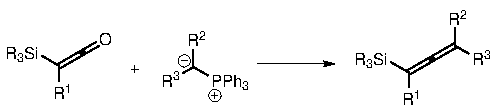
\includegraphics[width=8.2cm,keepaspectratio]{figure1}
%% \sglcolfigure{figure1}
\end{figure}

[\ldots]

\section{Results and Discussion}
Our investigations began with the preparation of substituted silylketenes \CN{1} as substrates for the alkylidenation chemistry. This was carried out under our previously reported conditions for rhodium(II) octanoate-mediated rearrangement of silyl diazoketones \CN{2}, which in turn were prepared by \textit{C}-silylation of the parent diazoketones \CN{3} with triethylsilyl triflate (\cref{scheme:1}). It should be noted that while the alkyl-substituted silylketenes are relatively stable and show little decomposition at room temperature over several days, the (hetero)aromatic-substituted silylketenes are much less robust and should be used quickly or stored in a freezer.

\begin{scheme}
\caption{Synthesis of substituted silylketenes \CN{1}.}
\label{scheme:1}
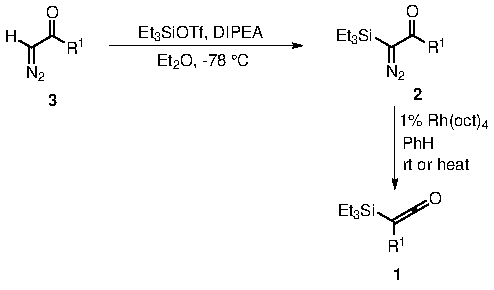
\includegraphics[width=8.2cm,keepaspectratio]{scheme1}
\end{scheme}

[\ldots]

With the requisite silylketenes in hand, attention turned to their reaction with the carboethoxy-stabilised phosphoranes \CN{4} and \CN{5}. At the outset, it was by no means certain that these would react efficiently with substituted silylketenes \CN{1} since it is well documented that nucleophiles attack silylketenes \textit{anti} to the silicon, i.e., the phosphoranes would be approaching from the same side as the \chem{R^1}-substituent. Since in all previous examples this substituent has been a hydrogen atom, the extension to bulkier substituents could not be taken for granted. In the event, however, we were pleased to find that in nearly all cases the desired allenylsilanes were formed in moderate to excellent yield (\cref{scheme:2}, \cref{tab:1}, see \cref{si:1} for full experimental data).
\begin{scheme}
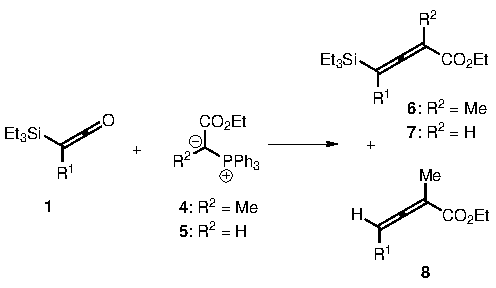
\includegraphics[width=8.2cm,keepaspectratio]{scheme2}
\caption{Reaction of substituted silylketenes with ester-stabilised phosphoranes.}
\label{scheme:2}
\end{scheme}
%%%%%%%%%%%%%%%%%%%%%%%%%%%%%%%%%%%%%%%%%%%%%%%%%%%%%%%%%%%%%%%%%%%%%
%% Tables are a bit special. Only there the \footnote is allowed for
%% Beilstein publications.
%%
%% As for figures and schemes sglcoltabular and dblcoltabular can be
%% used to get tables of the correct width. If you do not want to
%% messure the columns you can use parameter ``X'' of the tabularx
%% package for one column or more to get equal-sized columns.
%%%%%%%%%%%%%%%%%%%%%%%%%%%%%%%%%%%%%%%%%%%%%%%%%%%%%%%%%%%%%%%%%%%%%

\begin{table}
\caption{Reaction of substituted silylketenes with ester-stabilised phosphoranes.}
\label{tab:1}
\begin{dblcoltabularx}{|l|l|l|l|l|X|X|}\hline
\bfseries Entry & \bfseries Ketene & \bfseries Ylide & \bfseries Temp [\celsius] & \bfseries \textit{t} [h] & \bfseries Solvent & \bfseries Yield 6/7 (8)\\\hline
1 & \CN{1a} & \CN{4} & 80 & 24 & PhH & 54\,\%\\\hline
2 & \CN{1a} & \CN{5} & rt & 3  & \CHCL & 60\,\%\\\hline
3 & \CN{1b} & \CN{4} & 110 & 24 & toluene & 45\,\%\\\hline
4 & \CN{1b} & \CN{5} & reflux & 24 & \CHCL & 77\,\%\\\hline
5 & \CN{1c} & \CN{4} & 80 & 24 & PhH & 60\,\%\\\hline
6 & \CN{1c} & \CN{5} & rt & 6  & \CHCL & 81\,\%\\\hline
7 & \CN{1d} & \CN{4} & 110 & 48 & toluene & 22\,\%%
   \footnote{60\,\% of starting material recovered}\\\hline
8 & \CN{1d} & \CN{5} & 80 & 48 & toluene & 78\,\%\\\hline
9 & \CN{1e} & \CN{4} & 80 & 24 & PhH & 55\,\% (7\,\%)\\\hline
10 & \CN{1f} & \CN{4} & 60 & 5 & \CHCL & 44\,\% (3\,\%)\\\hline
11 & \CN{1h} & \CN{4} & rt & 6 & \CHCL & 0\,\% (57\,\%)\\\hline
12 & \CN{1h} & \CN{4} & 50 & 1 & \CHCL & 7\,\% (23\,\%)\\\hline
13 & \CN{1i} & \CN{4} & rt & 10 & \CHCL & 0\,\% (67\,\%)\\\hline
14 & \CN{1i} & \CN{5} & rt & 2 & \CHCL & 98\,\%\\\hline
15 & \CN{1j} & \CN{4} & 80 & 12 & PhH & 74\,\% (19\,\%)\\\hline
\end{dblcoltabularx}
\end{table}

As expected, reactions with the more substituted ylide \CN{4} were significantly slower than those with the parent ylide \CN{5} (compare reaction temperatures and times, entries 1, 3 and 5 versus entries 2, 4 and 6). [...]

%%%%%%%%%%%%%%%%%%%%%%%%%%%%%%%%%%%%%%%%%%%%%%%%%%%%%%%%%%%%%%%%%%%%%
%% The Supporting Information is an essential part of many articles.
%% They are given inside the ``suppinfo'' environment with the
%% \sifile command which gets the following mandatory arguments:
%% #1: File name
%% #2: File type
%% #3: Descriptive File title
%% A long description can be given using the optional argument.
%%
%% You can label each entry and reference it in the text.
%%%%%%%%%%%%%%%%%%%%%%%%%%%%%%%%%%%%%%%%%%%%%%%%%%%%%%%%%%%%%%%%%%%%%
\begin{suppinfo}
Supporting information features copies of \HNMR spectra of silylated diazoketones \CN{2} and silylketenes \CN{1}, plus \chem{{}^1H} and \CNMR spectra of allenylsilanes \CN{6}, \CN{7}, and \CN{14}--\CN{19}.
\sifile{S1.pdf}{PDF}{Experimental part}\label{si:1}
\sifile{S2.pdf}{PDF}{NMR spectra of compounds \CN{1}, \CN{2}, \CN{6} and \CN{7}}
\sifile{S3.pdf}{PDF}{NMR spectra of compounds \CN{14--19}}
\end{suppinfo}

%%%%%%%%%%%%%%%%%%%%%%%%%%%%%%%%%%%%%%%%%%%%%%%%%%%%%%%%%%%%%%%%%%%%%
%% The sections "Acknowledgements" and "Funding" can be given in all
%% manuscripts.
%% This should be done within the environments ``acknowledgements''
%% and ``funding'', which will produce the correct section titles.
%%%%%%%%%%%%%%%%%%%%%%%%%%%%%%%%%%%%%%%%%%%%%%%%%%%%%%%%%%%%%%%%%%%%%
\begin{acknowledgements}
We acknowledge Prof. H. Vlassov for the helpful discussions of the results and J. Martin for assistance with the synthesis.
\end{acknowledgements}

\begin{funding}
The following sources of funding are acknowledged: National Natural Science Foundation of China (S.P.M.; Grant Nos. 51502240, 11674273, U1856203), Wellcome Trust (S.P.M., Award No. 094542/Z/12/Z, EPSRC (P.C.D.; Grant No. GR/L60135/01 (PCD)), and both authors thank the generous research funding from Pfizer for financial support.
\end{funding}

%%%%%%%%%%%%%%%%%%%%%%%%%%%%%%%%%%%%%%%%%%%%%%%%%%%%%%%%%%%%%%%%%%%%%
%% The appropriate \bibliography command should be placed here.
%% Notice that the class file automatically sets \bibliographystyle
%% and also names the section correctly.
%%%%%%%%%%%%%%%%%%%%%%%%%%%%%%%%%%%%%%%%%%%%%%%%%%%%%%%%%%%%%%%%%%%%%
\bibliography{beilstein-template}

%%%%%%%%%%%%%%%%%%%%%%%%%%%%%%%%%%%%%%%%%%%%%%%%%%%%%%%%%%%%%%%%%%%%%
%% That's it. Ending the document finishes the article. Happy TeXing!
%%%%%%%%%%%%%%%%%%%%%%%%%%%%%%%%%%%%%%%%%%%%%%%%%%%%%%%%%%%%%%%%%%%%%
\end{document}
%</demo>
%\fi
